\documentclass[aps,prd,twocolumn,superscriptaddress,nofootinbib]{revtex4-2}
\usepackage{graphicx}
\usepackage{amsmath}
\usepackage{amssymb}
\usepackage{xcolor}
\usepackage{placeins}
\usepackage[hidelinks]{hyperref}
\newcommand{\github}{\raisebox{-0.35ex}{\includegraphics[height=2.0ex]{github_mark.pdf}}}
\renewcommand{\topfraction}{0.95}
\renewcommand{\bottomfraction}{0.6}
\renewcommand{\textfraction}{0.05}
\renewcommand{\floatpagefraction}{0.85}
\renewcommand{\dbltopfraction}{0.95}
\renewcommand{\dblfloatpagefraction}{0.5}
\setcounter{dbltopnumber}{3}
\graphicspath{{../figures/}}
\newcommand{\todo}[1]{\textcolor{red}{[#1]}}
\newcommand{\Mc}{\mathcal{M}_c}

\begin{document}

\title{When Do You Become a Stochastic Gravitational Wave Background? Revisited}

\author{Tore Boybeyi}
\affiliation{School of Physics and Astronomy, University of
Minnesota, Minneapolis, Minnesota 55455, USA}
\author{Vuk Mandic}
\affiliation{School of Physics and Astronomy, University of
Minnesota, Minneapolis, Minnesota 55455, USA}
\author{Joseph D. Romano}
\affiliation{Department of Physics and Astronomy, University of
Texas Rio Grande Valley, One West University Boulevard,
Brownsville, TX 78520, USA}

\date{\today}

\begin{abstract}
The astrophysical gravitational wave background in the terrestrial detector band consists of the signals of compact binary coalescences. The background divides into individually resolvable events and unresolvable subthreshold signals. The resolvable events are analyzed one at a time by sampling the posterior of a deterministic waveform, while the unresolvable part is searched with a summary statistic, the cross correlation of the detector pair weighted by the overlap reduction function. In this paper we ask how one moves from the summary statistic to the full event analysis as the number of retained statistics grows. We show that this passage is organized by generalized overlap reduction functions, contracted with cross moments of the matched filter outputs, which reduce to the standard overlap reduction function at the lowest order and recover the fully marginalized event likelihood in the untruncated limit. We demonstrate the method on individual events, where it reproduces the exact marginalized likelihood. We show that the standard overlap reduction function becomes non optimal already for signals with matched filter signal to noise ratio above 0.1, and that $O(100)$ statistics give a reliable stochastic search of the full subthreshold population. The method serves as an efficient and fast search for subthreshold and stochastic signals. We also demonstrate it on a simulated stochastic gravitational wave background and recover the merger rate and the mass distribution. We share the companion scripts and example notebooks at \href{https://github.com/dmatter1391/exmarg}{\github}.
\end{abstract}

\maketitle

\section{Introduction}

Today the stochastic gravitational wave background (SGWB) in the terrestrial detector band is expected to consist mostly of unresolvable compact binary coalescence (CBC) signals, which form an intermittent background \cite{Regimbau2011,MeacherThraneRegimbau,LVKO3iso}. Over the years various methodologies have been developed to search for it. Historically, the cross correlation statistic weighted by the overlap reduction function has been used \cite{Allen1999,Romano2017,LVKO3iso}, which assumes a continuous Gaussian background fully described by its mean spectrum. Later, the search was improved to account for the intermittent structure, through a mixture likelihood in which each data segment $d_i$ contains either noise or noise and a single signal \cite{Drasco2003},
\begin{equation}
\mathcal{L}(\{d\}) = \prod_i \big[ (1 - \xi)\, \mathcal{L}_n(d_i)
+ \xi\, \mathcal{L}_s(d_i) \big],
\label{eq:mix}
\end{equation}
with $\xi$ the probability that a segment holds a signal, and $\mathcal{L}_n$ and $\mathcal{L}_s$ the noise and signal likelihoods. Currently, two competing models build on this intermittent structure. One is the ``optimal'' search developed by Smith and Thrane \cite{Smith2018}, in which $\mathcal{L}_s$ is the evidence of a deterministic waveform marginalized over all of its parameters, recently demonstrated on a mock data challenge \cite{Kou2025}. The other is the stochastic search for intermittent backgrounds \cite{Lawrence2023}, which models $\mathcal{L}_s$ with a stochastic amplitude instead of a waveform. Underlying all of these methods sits the question posed by Cornish and Romano~\cite{CornishRomano2015}, when is a gravitational wave signal stochastic, which they answered through Bayesian model selection between a deterministic and a stochastic model. We revisit their question at the level of the likelihood, where the answer becomes a continuous family rather than a binary choice.

Intuitively, for a weak signal $\mathcal{L}_s$ is a nearly flat surface over the signal parameters, so it should admit an expansion in terms of a small number of summary statistics, which is why the cross correlation is nearly optimal in this limit. For a loud signal the surface is sharply peaked at the true parameters, and only the full event analysis resolves the peak. In this paper we work out the transition between the two regimes, order by order in the signal to noise ratio (SNR). We build on our recent work \cite{companion}, where we showed that infinitely many different interpolations are possible between the exact likelihood and the cross correlation statistic, through different coarse grainings of the characteristic function of the gravitational wave strain in multiple detectors, with the most ``efficient'' statistics being those along which the characteristic function changes most steeply. This paper gives the concrete implementation of one such interpolation for a compact binary signal in two detectors, as a practical search pipeline.

In particular, we showed that the behaviour of the characteristic function of the strain, $\Phi(J_{I,\nu})$, with one argument $J_{I,\nu}$ for each detector $I$ and frequency bin $\nu$, near the origin $J_{I,\nu} = 0$ is related to the correlations among the different frequency bins, and that its higher order derivatives at the origin correspond to generalized overlap reduction functions. The second derivative gives the rank two $\Gamma^{(2)}_{IJ}(f)$ of the standard search, the fourth derivative gives $\Gamma^{(4)}_{IJKL}(f, f', f'')$, which carries 3 frequencies and 4 detector indices, and each further order adds two frequencies and two detector indices. These correlations grow combinatorially with the order, which has held the previous works searching for non Gaussianities or higher moments of the background to the 4 point function \cite{Thrane2013,MartelliniRegimbau2014,Seto2009}. The growth is only an artifact of the frequency bin picture. For example, the fourth power of the matched filter output $z(t) = \sum_\nu z_\nu\, e^{2\pi i \nu t / T}$, integrated over the segment, couples every quadruple of bins under one frequency constraint yet is a single one dimensional integral,
\begin{equation}
\frac{1}{T} \int_0^T dt\, |z(t)|^4 =
\sum_{\nu_a - \nu_b + \nu_c - \nu_d = 0}
z_{\nu_a} \bar z_{\nu_b} z_{\nu_c} \bar z_{\nu_d}.
\label{eq:fourpoint}
\end{equation}
We show that a similar idea, the collapse of the frequency sums onto time domain integrals of the matched filter output, can also be used for the whole marginalized likelihood at every order, which we detail shortly.

The plan of this paper is as follows. Section~\ref{sec:method} derives the interpolation, from the marginalized likelihood of a single compact binary in two detectors to a series of generalized overlap reduction functions contracted with per template data integrals. Section~\ref{sec:validation} validates the series on individual events against the exact likelihood, and measures how many terms a signal of a given SNR requires. Section~\ref{sec:population} applies the method to a simulated intermittent background and recovers the merger rate and the mass distribution, and Section~\ref{sec:conclusion} concludes.

Throughout the derivation the two detectors are labeled $I = 1, 2$ and are allowed arbitrary stationary Gaussian noise spectra $S_I(f)$. The numerical background study uses the LIGO Hanford and LIGO Livingston A+ design sensitivity of Sec.~\ref{sec:population}. A data segment of duration $T$ has frequency bins $f_\nu = \nu / T$, data $\tilde d_{I,\nu}$, and noise variance $\sigma^2_{I,\nu} = T S_I(f_\nu) / 2$ per complex bin. The intrinsic parameters of the binary are collected as $\vec\lambda = (\Mc, q, \chi_{\rm eff})$, the chirp mass, the mass ratio, and one aligned spin of an equal aligned spin waveform. The extrinsic parameters are collected as $\vec\theta$, the sky direction $\hat n$, the arrival time $t$, the overall phase $\varphi_0$, the polarization angle $\psi$, the inclination cosine $\chi$, and the distance scale $y = D_0 / D$ at a reference distance $D_0$. We assume the IMRPhenomXAS waveform \cite{XAS}, a dominant mode aligned spin model, but our method is general and can be straightforwardly extended to other waveform models, to higher harmonics and precession through additional mode tables, and to unequal detector noise.

\section{Method}
\label{sec:method}

We search for the intermittent background with the mixture likelihood of Eq.~\eqref{eq:mix}, with the Poisson probabilities of the event count of a segment as the weights,
\begin{equation}
\mathcal{L}(\{d\} \mid \bar N) = \prod_i \Big[
e^{-\bar N}\, \mathcal{L}_n(d_i)
+ \bar N e^{-\bar N}\, \mathcal{L}_s(d_i) \Big],
\label{eq:mixture}
\end{equation}
where $\bar N = R_0 V T_{\rm seg}$ is the mean number of events per segment, set by the merger rate density $R_0$, the volume $V$ of the distance prior, and the exposure $T_{\rm seg}$. The same exposure enters the event generation and the mean $\bar N$, so the recovered rate is consistent with the injected one. For now we consider the rare event regime $\bar N \ll 1$, so a segment carries at most one event and the signal likelihood is an integral over the parameters of a single source,
\begin{equation}
\mathcal{L}_s(d) = \int d\vec\lambda\; \pi(\vec\lambda)
\int d\vec\theta\; \pi(\vec\theta)\;
\mathcal{L}(d \mid \vec\theta, \vec\lambda).
\label{eq:ls}
\end{equation}
The generalization to overlapping events, through the full Poisson sum over the event count, is shown in the companion paper \cite{companion}. We choose isotropic priors in all angles and a distance prior uniform in Euclidean volume, $p(D) = 3 D^2 / D_{\max}^3$ for $D \le D_{\max}$, which in the amplitude variable $y$ reads $p(y) = 3 y_{\min}^3 / y^4$ for $y \ge y_{\min} = D_0 / D_{\max}$.

The single event likelihood ratio in the integrand of
Eq.~\eqref{eq:ls} is Gaussian and, in the frequency domain, sums
over the bins of the two detectors,
\begin{equation}
\ln \frac{\mathcal{L}(d \mid \vec\theta, \vec\lambda)}
{\mathcal{L}_n(d)}
= \sum_{I=1,2} \sum_\nu
\frac{2\, \mathrm{Re}[ \tilde d^{*}_{I,\nu} \tilde h_{I,\nu} ]
- |\tilde h_{I,\nu}|^2}{\sigma^2_{I,\nu}},
\label{eq:lnratio}
\end{equation}
with the two detector template
\begin{equation}
\begin{aligned}
\tilde h_{I,\nu} &= y\, R_I(\hat n, \psi, \chi)\, e^{-i\varphi_0}\,
a_\nu(\vec\lambda) \\
&\quad \times e^{i\Psi_0(f_\nu, \vec\lambda)}\,
e^{-2\pi i f_\nu ( t + \tau_I(\hat n) )}, \\
\tau_I(\hat n) &= \frac{\hat n \cdot (\vec x_I - \vec x_2)}{c},
\end{aligned}
\label{eq:template}
\end{equation}
where $\vec x_I$ is the detector position and $\tau_2 = 0$. The
response of detector $I$ to the sky direction $\hat n$, the
polarization angle $\psi$, and the inclination variable $\chi$
is
\begin{equation}
R_I(\hat n, \psi, \chi) = \frac{1 + \chi^2}{2}\,
F^I_+(\hat n, \psi) + i\, \chi\, F^I_\times(\hat n, \psi),
\label{eq:response}
\end{equation}
with the antenna patterns $F^I_+$ and $F^I_\times$, and
$a_\nu(\vec\lambda)$ and $\Psi_0(f_\nu, \vec\lambda)$ are the
amplitude and phase of the waveform at the fiducial distance
$D_0$. We substitute
Eq.~\eqref{eq:template} into Eq.~\eqref{eq:lnratio} term by
term. In the linear term the response, the coalescence phase,
and the amplitude scale carry no frequency index and move out of
the sum over the bins,
\begin{align}
\sum_\nu
\frac{2\, \mathrm{Re}[ \tilde d^{*}_{I,\nu} \tilde h_{I,\nu} ]}
{\sigma^2_{I,\nu}}
&= 2 y\, \mathrm{Re}\Big[ R_I(\hat n, \psi, \chi)\,
e^{-i\varphi_0}\notag\\
&\times \sum_\nu\!
\frac{\tilde d^{*}_{I,\nu}}{\sigma^2_{I,\nu}}
a_\nu(\vec\lambda) e^{i \Psi_0(f_\nu, \vec\lambda)}
e^{-2\pi i f_\nu (t + \tau_I)}\!\Big],
\label{eq:linstep}
\end{align}
and the remaining sum is a discrete Fourier series in the time
$t + \tau_I$, since $f_\nu = \nu / T$. In the quadratic term
every phase carries unit modulus and drops,
\begin{equation}
\sum_\nu \frac{|\tilde h_{I,\nu}|^2}{\sigma^2_{I,\nu}}
= y^2\, |R_I(\hat n, \psi, \chi)|^2
\sum_\nu \frac{a_\nu(\vec\lambda)^2}{\sigma^2_{I,\nu}}.
\label{eq:quadstep}
\end{equation}
We name the two frequency sums, the matched filter series and
the template power of detector $I$,
\begin{equation}
\begin{aligned}
z_I(t, \vec\lambda) &= \sum_\nu
\frac{\tilde d^{*}_{I,\nu}\, a_\nu(\vec\lambda)\,
e^{i \Psi_0(f_\nu, \vec\lambda)}}
{\sigma^2_{I,\nu}}\, e^{-2\pi i \nu t / T},\\
u_I(\vec\lambda) &= \sum_\nu
\frac{a_\nu(\vec\lambda)^2}{\sigma^2_{I,\nu}},
\end{aligned}
\label{eq:zu}
\end{equation}
so the sum of Eq.~\eqref{eq:linstep} and
Eq.~\eqref{eq:quadstep} over the two detectors reduces the log
ratio of Eq.~\eqref{eq:lnratio} to
\begin{equation}
\ln \frac{\mathcal{L}(d \mid \vec\theta, \vec\lambda)}
{\mathcal{L}_n(d)}
= 2 y\, \mathrm{Re}\big[ e^{-i\varphi_0}\, Z \big] - y^2 A,
\label{eq:reduced}
\end{equation}
with the coherent combination and the orientation weight
\begin{equation}
\begin{aligned}
Z(t, \hat n, \psi, \chi, \vec\lambda)
&= R_1\, z_1(t + \tau(\hat n), \vec\lambda)
+ R_2\, z_2(t, \vec\lambda),\\
A(\hat n, \psi, \chi, \vec\lambda)
&= |R_1|^2\, u_1(\vec\lambda)
+ |R_2|^2\, u_2(\vec\lambda),
\end{aligned}
\label{eq:ZA}
\end{equation}
and $\tau(\hat n) = \tau_1(\hat n) = \hat n \cdot \Delta \vec x / c$
the inter detector delay for
$\Delta \vec x = \vec x_1 - \vec x_2$. Marginalizing over the
extrinsic parameters with their priors, and writing every integral
explicitly, the extrinsic marginalized likelihood ratio at fixed
intrinsic parameters, $\Lambda(\vec\lambda)$, is
\begin{widetext}
\begin{equation}
\Lambda(\vec\lambda) = \frac{1}{4\pi} \int d\Omega\,
\frac{1}{2\Delta t} \int_{t_c - \Delta t}^{t_c + \Delta t} dt\,
\frac{1}{\pi} \int_0^\pi d\psi\,
\frac{1}{2} \int_{-1}^1 d\chi
\int_{y_{\min}}^\infty dy\, p(y)\,
\frac{1}{2\pi} \int_0^{2\pi} d\varphi_0\,
\exp\!\big( 2 y\, \mathrm{Re}[ e^{-i\varphi_0} Z ] - y^2 A \big).
\label{eq:marg}
\end{equation}
\end{widetext}
The intrinsic integral of Eq.~\eqref{eq:ls} is not yet taken here,
$\mathcal{L}_s / \mathcal{L}_n = \int d\vec\lambda\,
\pi(\vec\lambda)\, \Lambda(\vec\lambda)$, and it is carried out
in Sec.~\ref{sec:population} as a weighted sum over a template grid.
The overall phase enters only
through $\mathrm{Re}[ e^{-i\varphi_0} Z ]$ and $Z$ does not depend
on $\varphi_0$, so the uniform phase integral is a Bessel function
\cite{DLMF},
\begin{equation}
\frac{1}{2\pi} \int_0^{2\pi} d\varphi_0\,
e^{2 y\, \mathrm{Re}[ e^{-i\varphi_0} Z ]} = I_0( 2 y |Z| ),
\label{eq:bessel}
\end{equation}
which depends on the data only through the magnitude $|Z|$.

The argument $2 y |Z|$ of this Bessel function grows as the squared
matched filter SNR. The template of Eq.~\eqref{eq:template} carries
the optimal SNR
\begin{equation}
\rho^2(y) = 2 \sum_{I,\nu}
\frac{|\tilde h_{I,\nu}(\vec\theta, \vec\lambda)|^2}{\sigma^2_{I,\nu}}
= 2 A y^2,
\label{eq:rho}
\end{equation}
and a matched signal shifts the mean of $|Z|$ to $y A$, giving
$y |Z| \simeq A y^2 = \rho^2(y) / 2$, measured from the data by
$\rho_{\rm mf} = \sqrt{2}\, |Z| / \sqrt{A}$. The argument is thus
small in the subthreshold regime, and we expand the Bessel function,
truncating at order $n_{\max}$,
\begin{equation}
I_0(2 y |Z|) \simeq \sum_{n=0}^{n_{\max}}
\frac{(y |Z|)^{2n}}{(n!)^2},
\label{eq:taylor}
\end{equation}
with exact coefficients. The expansion is of the ratio itself rather
than of its logarithm, because only the ratio can be marginalized term
by term under the integrals of Eq.~\eqref{eq:marg}. Each retained
power $(y |Z|)^{2n}$ becomes a computable statistic below, and the
choice of $n_{\max}$ is tested in Sec.~\ref{sec:validation}.

\begin{figure*}[!t]
\centering
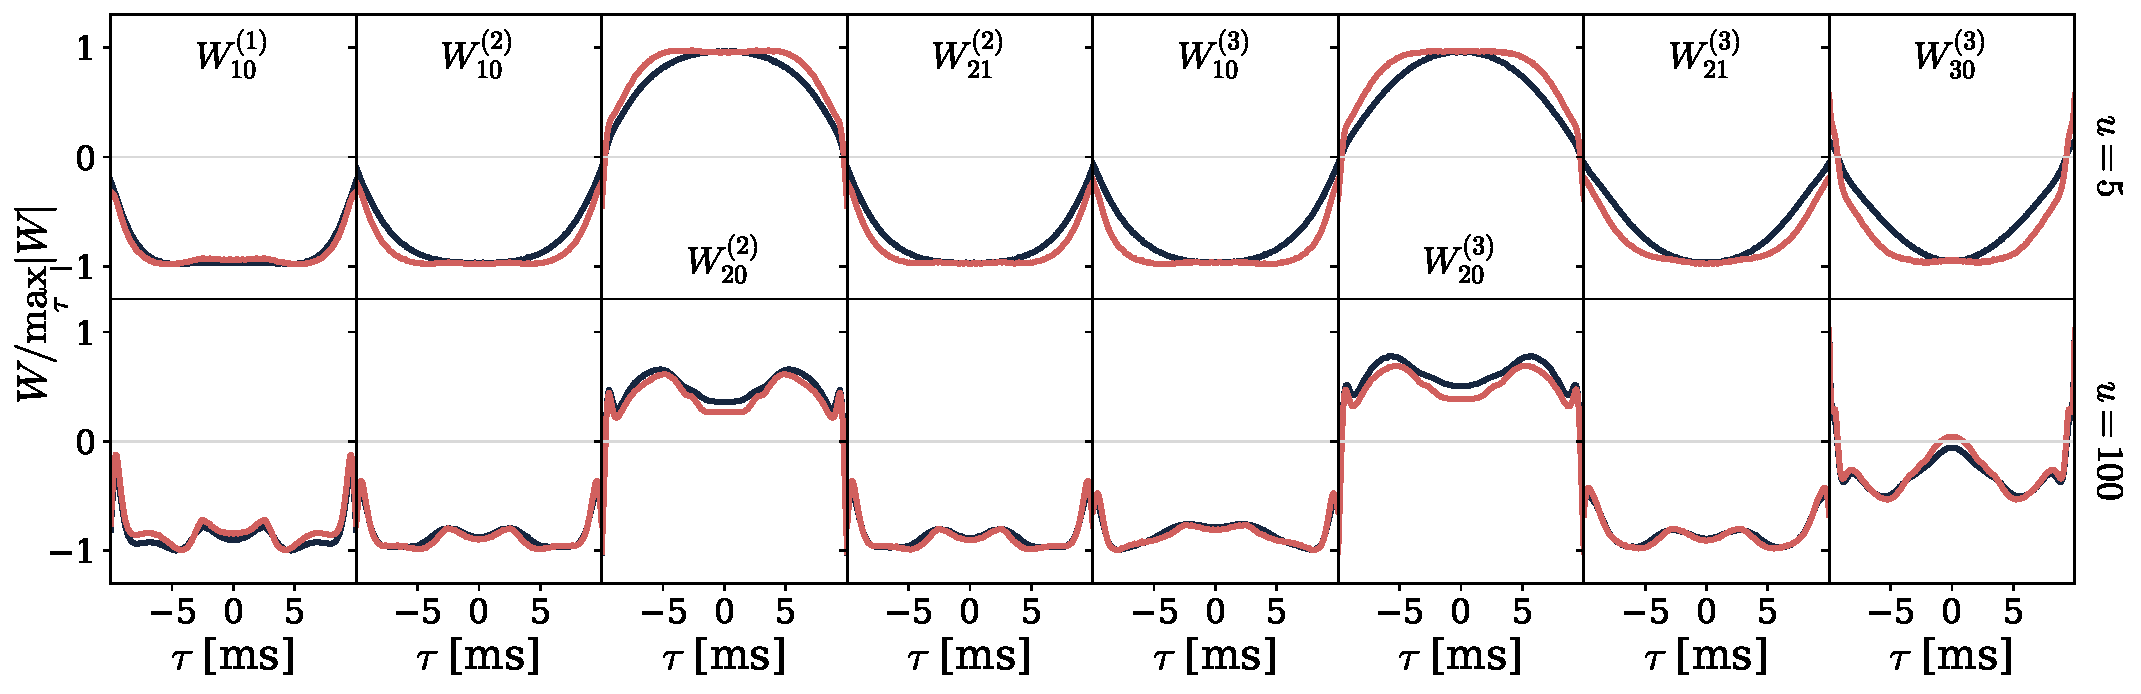
\includegraphics[width=\textwidth]{W_family.pdf}\\[4pt]
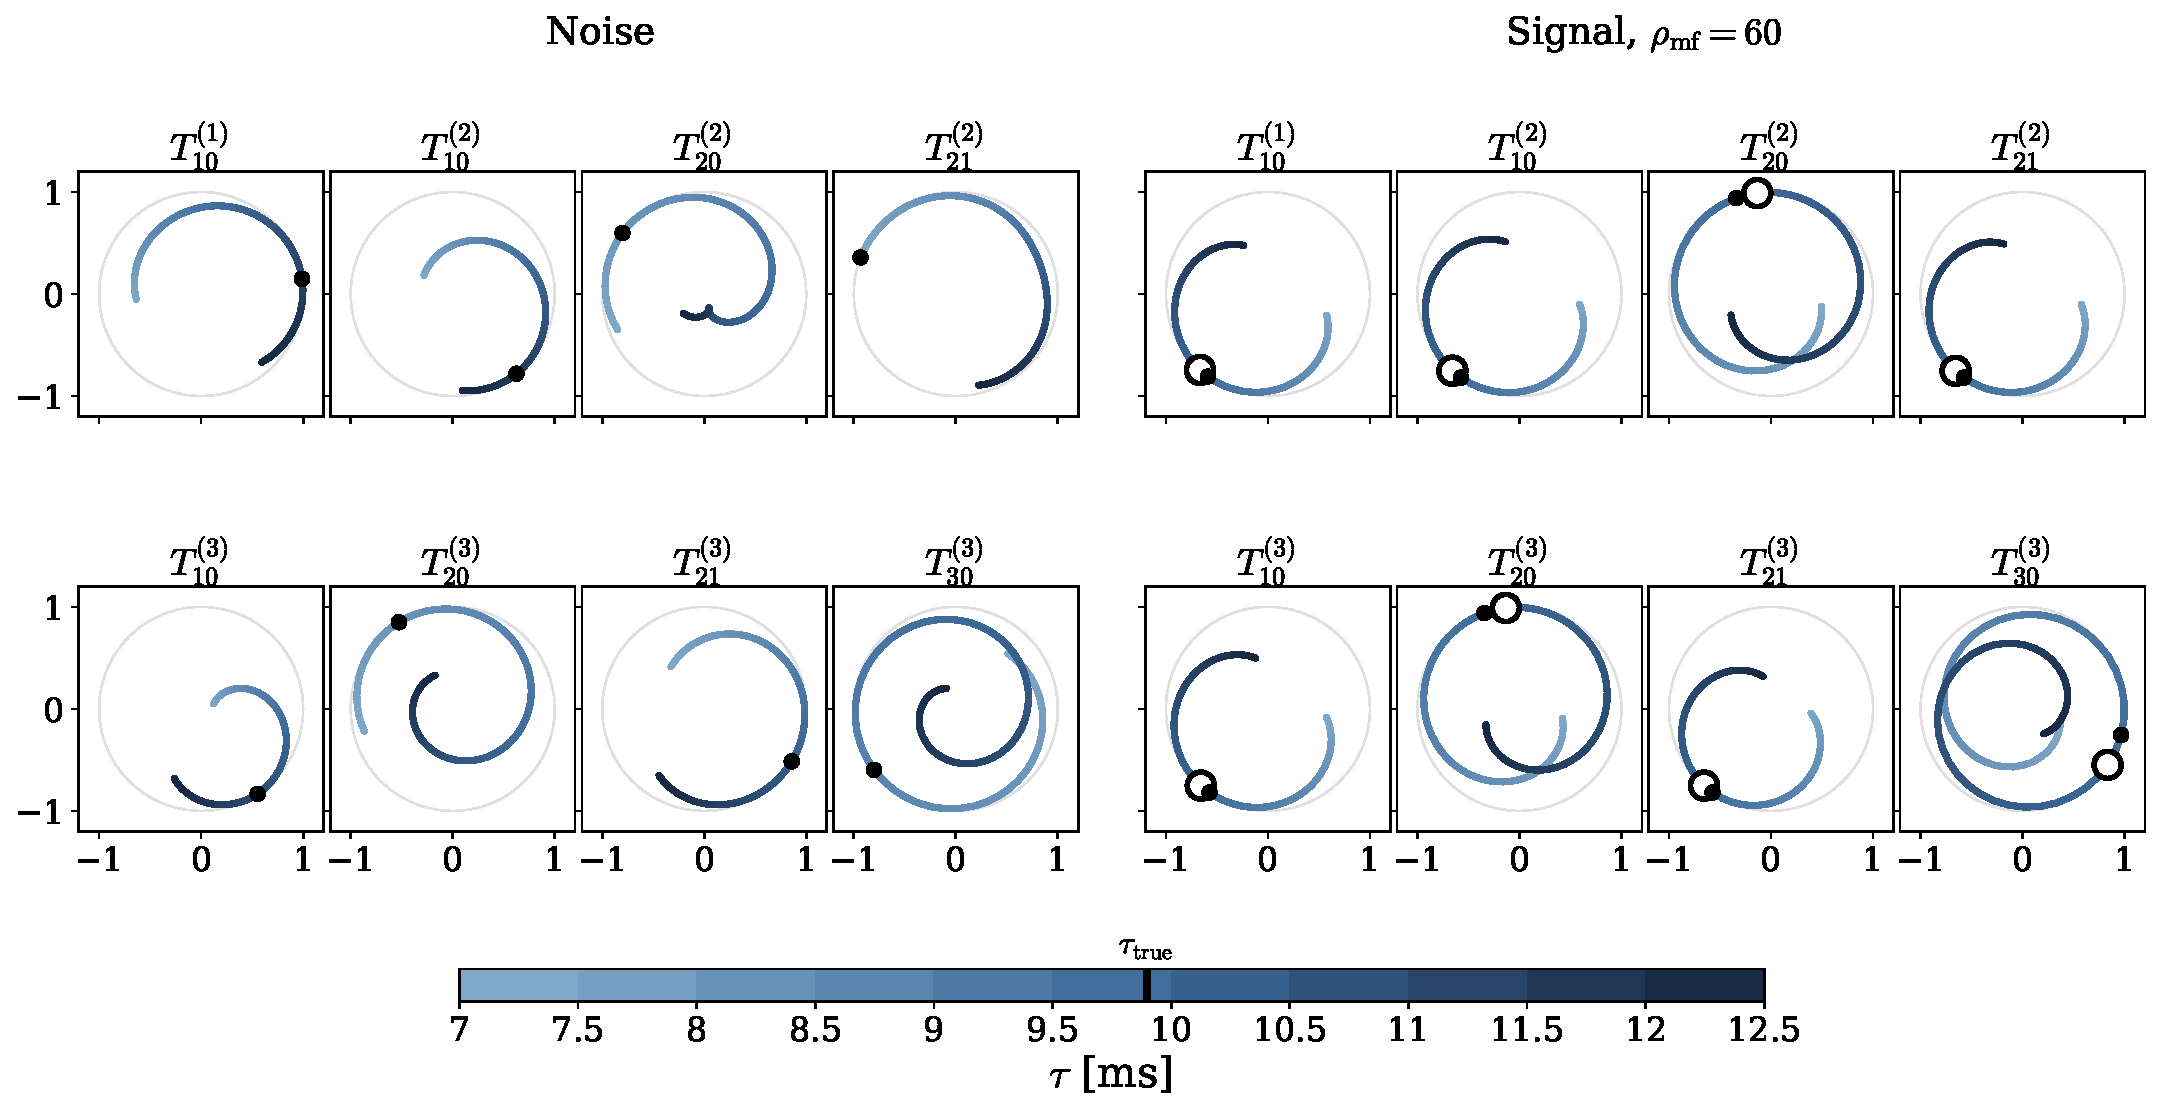
\includegraphics[width=\textwidth]{T_family.pdf}
\caption{The two quantities of
Eq.~\eqref{eq:master}. Top, the normalized geometric factors
$W^{(n)}_{ab}(\tau, u_1, u_2)$ for two values of the template power
(rows) and two distance priors, uniform in volume
($p(D) \propto D^2$, dark) and uniform in distance
($p(D) \propto 1$, red), supported on the delay range
$|\tau| \le |\Delta \vec x| / c \approx 10$ ms, the light travel
time between the detectors. Bottom, the normalized data integrals
$T^{(n)}_{ab}(\tau, \vec\lambda)$ of a noise segment (left half)
and an injected event (right half), each curve scaled to its own
maximum. The right half is evaluated at the true intrinsic
template, $\vec\lambda = \vec\lambda_{\rm true}$. There the
magnitude $|T^{(n)}_{ab}(\tau, \vec\lambda_{\rm true})|$ is maximal
at the true inter detector delay, where the matched filter outputs
of the two detectors line up. The black dots mark the delay of each
curve's maximum and the open circles mark the true delay. Under
noise the curves peak at random delays.}
\label{fig:tables}
\end{figure*}

Take the first order of the expansion. Its contribution to
Eq.~\eqref{eq:marg} is the average of $y^2 |Z|^2$ over the extrinsic
parameters. The distance integral gives
$\int_{y_{\min}}^\infty dy\, p(y)\, y^2\, e^{-y^2 A} = M_1(A)$,
and the square opens by Eq.~\eqref{eq:ZA} into 4 monomials,
\begin{equation}
|Z|^2 = |R_1|^2 z_1 \bar z_1 + |R_2|^2 z_2 \bar z_2
+ R_1 \bar R_2 z_1 \bar z_2 + \bar R_1 R_2 \bar z_1 z_2,
\label{eq:binom1}
\end{equation}
with $z_1$ evaluated at $t + \tau(\hat n)$ and $z_2$ at $t$. Each
monomial is an orientation factor times a data factor. We take the
cross monomial $R_1 \bar R_2\, z_1 \bar z_2$ as the example and
follow it through the integrals of Eq.~\eqref{eq:marg}. The
distance integral gives the moments
$M_n(A) = \int_{y_{\min}}^\infty dy\, p(y)\, y^{2n} e^{-y^2 A}$,
evaluated in closed form in Appendix~\ref{app:construction}, here
at $n = 1$, and the contribution of the monomial reads
\begin{align}
&\frac{1}{4\pi}\!\int\! d\Omega\,
\frac{1}{\pi}\!\int_0^\pi\! d\psi\,
\frac{1}{2}\!\int_{-1}^{1}\! d\chi\;
M_1\big(A(\hat n, \psi, \chi)\big)\, R_1 \bar R_2\notag\\
&\;\times \frac{1}{2\Delta t}\!
\int_{t_c-\Delta t}^{t_c+\Delta t}\! dt\;
z_1(t + \tau(\hat n), \vec\lambda)\,
\bar z_2(t, \vec\lambda).
\label{eq:crossterm}
\end{align}
The orientation integrals cannot be carried out on their own,
because the sky direction also sits inside the data factor,
through the delay $\tau(\hat n)$ of $z_1$. We insert the
identity
$1 = \int d\tau\, \delta( \tau - \hat n \cdot \Delta \vec x / c )$
under the orientation average and exchange the order of the
integrals,
\begin{align}
\text{Eq.}~\eqref{eq:crossterm}
&= \int\! d\tau
\Big\langle \delta\big( \tau -
\tfrac{\hat n \cdot \Delta \vec x}{c} \big)\,
M_1(A)\, R_1 \bar R_2 \Big\rangle_{\hat n, \psi, \chi}
\notag\\
&\;\times \frac{1}{2\Delta t}\!
\int_{t_c-\Delta t}^{t_c+\Delta t}\! dt\;
z_1(t + \tau, \vec\lambda)\, \bar z_2(t, \vec\lambda).
\label{eq:split}
\end{align}
The first line only depends on the geometry (and the distance
prior). Therefore it can be precomputed and tabulated, and it is
the kernel $W^{(1)}_{10}(\tau, u_1, u_2)$ of Eq.~\eqref{eq:W}
below. The second line only depends on the data and the delay
$\tau$, and it no longer knows the sky direction. We can extend
this to the higher order terms with the binomial expansion of the
retained power,
\begin{align}
|Z|^{2n} = \sum_{a=0}^{n}\sum_{b=0}^{n}
\binom{n}{a}\binom{n}{b}\,
& R_1^{a} \bar R_1^{b} R_2^{n-a} \bar R_2^{n-b}\notag\\
\times\; z_1^{a} \bar z_1^{b}(t + \tau(\hat n))\,
& z_2^{n-a} \bar z_2^{n-b}(t).
\label{eq:binomn}
\end{align}
The truncated likelihood ratio therefore collects into
\begin{equation}
\begin{aligned}
\Lambda(\vec\lambda) = \sum_{n=0}^{n_{\max}} \frac{1}{(n!)^2}
\sum_{a=0}^{n} \sum_{b=0}^{n} & \binom{n}{a} \binom{n}{b} \\
\times \int d\tau\, & W^{(n)}_{ab}(\tau, u_1, u_2)\,
T^{(n)}_{ab}(\tau, \vec\lambda),
\end{aligned}
\label{eq:master}
\end{equation}
which is the main result of this paper. The data integral
\begin{equation}
T^{(n)}_{ab}(\tau, \vec\lambda) = \frac{1}{2\Delta t}
\int_{t_c - \Delta t}^{t_c + \Delta t} dt\,
z_1^{a} \bar z_1^{b}(t + \tau)\, z_2^{n-a} \bar z_2^{n-b}(t),
\label{eq:T}
\end{equation}
averaged over the arrival window of half width $\Delta t$ around the
segment center $t_c$, with $\Delta t$ chosen so that the longest
template of the bank stays inside the segment, is the delayed cross
moment of the
matched filter outputs $z_I(t)$ of the two detectors, the signal to
noise series whose peak marks a candidate arrival time. The
$T^{(n)}_{ab}$ are complex quantities, generalized matched filters
(or generalized cross correlations) of the two detector data, and
they depend on the
assumed intrinsic template $\vec\lambda$ through the matched filter
outputs. The order $n$
is the total power of the matched filter outputs carried by the term.
The geometric factor is the orientation and distance average of the
detector responses at fixed delay,
\begin{equation}
\begin{aligned}
W^{(n)}_{ab}(\tau, u_1, u_2) = \Big\langle
& M_n(A)\, R_1^{a} \bar R_1^{b} R_2^{n-a} \bar R_2^{n-b} \\
& \times \delta\big( \tau - \tfrac{\hat n \cdot \Delta \vec x}{c} \big)
\Big\rangle_{\hat n, \psi, \chi},
\end{aligned}
\label{eq:W}
\end{equation}
or openly as
\begin{align}
W^{(n)}_{ab}&(\tau, u_1, u_2)
= \frac{1}{4\pi}\!\int\! d\Omega\,
\frac{1}{\pi}\!\int_0^\pi\! d\psi\,
\frac{1}{2}\!\int_{-1}^{1}\! d\chi\notag\\
&\times M_n\big( |R_1|^2 u_1 + |R_2|^2 u_2 \big)\notag\\
&\times R_1^{a} \bar R_1^{b} R_2^{n-a} \bar R_2^{n-b}\,
\delta\big( \tau - \tfrac{\hat n \cdot \Delta \vec x}{c} \big),
\label{eq:Wopen}
\end{align}
with the distance moment $M_n$ defined above. The delta function
restricts the sky average to the ring of constant inter detector
delay, so $W^{(n)}_{ab}$ lives on the delay rings of the sky.
Coincidentally, in Ref.~\cite{cogwheel} the proposal
distributions for the sky location were chosen along the same
rings of constant delay. In our framework we can see that
$W^{(n)}_{ab}$ emerges as the natural object of the extrinsic
marginalization along these rings. It is a real
quantity, and it depends on the
template only through the two template powers $(u_1, u_2)$. The top
panels of Fig.~\ref{fig:tables} show it for the LIGO Hanford and LIGO
Livingston detectors.



\begin{figure}[!t]
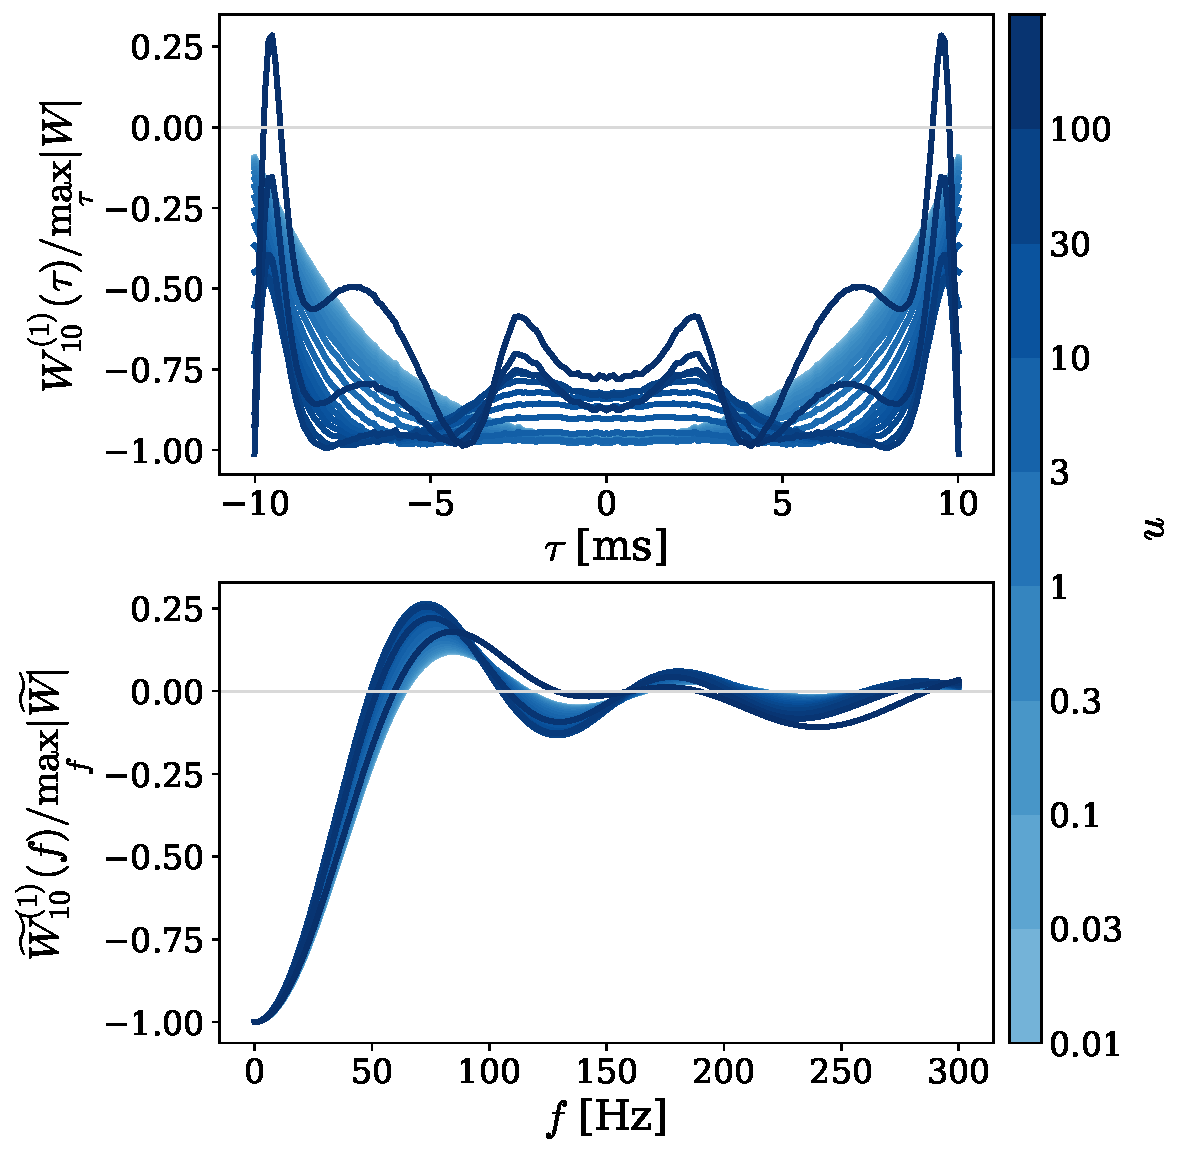
\includegraphics[width=\columnwidth]{W_u0.pdf}
\caption{The generalized overlap reduction function. The
Fourier transform of $W^{(1)}_{10}$ for a range of
template power values reproduces the standard function in the weak
signal limit and deforms away from it.}
\label{fig:oru}
\end{figure}

The Fourier transform of $W^{(n)}_{ab}$ in the delay gives
the overlap reduction function. In the zero template power limit
$W^{(1)}_{10}$ reproduces the function of Allen and Romano
\cite{Allen1999}, with its first zero near 64 Hz for the Hanford and
Livingston pair,
\begin{equation}
\Gamma^{(2)}_{12}(f) \propto \int d\tau\, e^{-2\pi i f \tau}\,
W^{(1)}_{10}(\tau, u_1, u_2)\big|_{u_1, u_2 \to 0}.
\label{eq:orf2}
\end{equation}
At non-zero template power the overlap reduction function deforms, so the cross-correlation statistic is already non-optimal for $\rho_{\rm mf} \gtrsim 0.1$, where the eigenvalue spectrum broadens beyond a single mode (Appendix~\ref{app:modes}). A similar effect was seen in a mock data study of the astrophysical background \cite{MeacherThraneRegimbau}, where a single realization gave a cross spectrum that departs from the idealized overlap reduction function even though it agrees with it on average. Figure~\ref{fig:oru} shows $W^{(1)}_{10}$ transformed to the frequency domain, which reproduces the standard overlap reduction function in the weak signal limit and deforms away from it as the template power grows.

The $n = 0$ term
carries no data, $\int d\tau\, W^{(0)}_{00}(\tau, u_1, u_2) =
\langle M_0(A) \rangle$, and sets the baseline of an empty segment.
At $n = 1$ the index pairs $(a, b) = (1, 1)$ and $(0, 0)$ give the
auto powers of the two detectors, and the pair $(1, 0)$, with its
conjugate $(0, 1)$, gives the cross correlation,
\begin{equation}
\begin{aligned}
\Lambda^{(1)} = \int d\tau\, \Big[\,
& W^{(1)}_{11}(\tau, u_1, u_2)\, \langle |z_1|^2 \rangle_t \\
& + W^{(1)}_{00}(\tau, u_1, u_2)\, \langle |z_2|^2 \rangle_t \\
& + 2\, W^{(1)}_{10}(\tau, u_1, u_2)\, \mathrm{Re}\, T^{(1)}_{10}(\tau)
\Big],
\end{aligned}
\label{eq:order1}
\end{equation}
with $T^{(1)}_{11} = \langle |z_1|^2 \rangle_t$ and
$T^{(1)}_{00} = \langle |z_2|^2 \rangle_t$ independent of the delay
and $T^{(1)}_{10}(\tau) = \langle z_1(t + \tau)\, \bar z_2(t)
\rangle_t$. These are the statistics of the classical searches, the
excess power of each detector and the cross correlation of the pair,
weighted across the delay by $W^{(1)}_{10}$. At $n = 2$ the series
adds the auto moments $\langle |z_I|^4 \rangle_t$, the intensity
cross correlation $T^{(2)}_{11}(\tau) =
\langle |z_1(t + \tau)|^2\, |z_2(t)|^2 \rangle_t$, and the coherent
pair term $T^{(2)}_{20}(\tau) =
\langle z_1^2(t + \tau)\, \bar z_2^2(t) \rangle_t$, which correlates
the two detectors at twice the phase of the chirp, together with
mixed products of the type
$|z_1(t + \tau)|^2\, z_1(t + \tau)\, \bar z_2(t)$. The higher orders
continue this pattern.

The truncated series is a finite order score that approaches the
marginalized likelihood ratio from below, since each term is positive
and the truncation discards the tail of the series. The discarded
weight can be restored as a truncation normalization. The normalized
version $\Lambda^\star$ is constructed and discussed in
Appendix~\ref{app:norm}, and we use it throughout. For the $n_{\max}$
adopted in this work the impact of the normalization is negligible in
the scenarios considered here.

In our pipeline the factors $W^{(n)}_{ab}(\tau, u_1, u_2)$ are
built once, up to $n_{\max}$, on the $(u_1, u_2)$ grid, and
their convergence with the resolution of the orientation
quadrature is shown in Appendix~\ref{app:construction}. The
quadrature can therefore be made much finer than what a
stochastic sampler, which repeats the sky integral at every
likelihood evaluation, can practically afford. We can then form
the following quantity that again does not involve any data,
\begin{equation}
\begin{aligned}
\mathcal{S}^{(n)}(\tau, z_1, z_2) = {} & \frac{1}{(n!)^2}
\sum_{a=0}^{n} \sum_{b=0}^{n} \binom{n}{a} \binom{n}{b} \\
& \times W^{(n)}_{ab}(\tau, u_1, u_2)\,
|z_1|^{a+b}\, |z_2|^{2n-a-b} \\
& \times \cos[(a-b)\, \Delta\varphi],
\end{aligned}
\label{eq:kernelS}
\end{equation}
with $\Delta\varphi = \arg( z_1 \bar z_2 )$. We also sum over
the orders,
$\mathcal{S} = \sum_{n \le n_{\max}} \mathcal{S}^{(n)}$. We
therefore only store this object at every
$(\tau, |z_1|, |z_2|, \Delta\varphi)$, which takes 0.4 GB per
point of the $(u_1, u_2)$ grid at run time. At run time each template $\vec\lambda$
requires only its matched filter series $z_I(t, \vec\lambda)$, built
from the data $\tilde d_{I,\nu}$ and the noise spectra $S_I(f)$, and
its template powers $u_I(\vec\lambda)$, built from the waveform and
the same spectra, both through Eq.~\eqref{eq:zu}. $\mathcal{S}$ is read at these
values, and the marginalized likelihood ratio is
assembled as
\begin{equation}
\Lambda(\vec\lambda) = \frac{1}{2\Delta t} \int dt \int d\tau\,
\mathcal{S}\big(\tau, z_1(t + \tau, \vec\lambda),
z_2(t, \vec\lambda)\big),
\label{eq:read}
\end{equation}
one read per template, so a full template grid is scanned in
parallel.

The truncation order is validated on single events in Appendix~\ref{sec:validation}. It reproduces the exact likelihood over the controlled range $\rho_{\rm mf} \lesssim \sqrt{2 n_{\max}}$, and the recovered posteriors are unbiased over 592 injections, with KS $p$ values of 0.28 to 0.87. Figure~\ref{fig:lnlmax} shows the truncated $\ln \Lambda$ against the truncation order at fixed matched filter SNRs. Each curve saturates once $n_{\max}$ passes the largest term of the series at $n \simeq \rho_{\rm mf}^2 / 2$, so the controlled range grows as $\sqrt{2 n_{\max}}$.

\begin{figure}[!t]
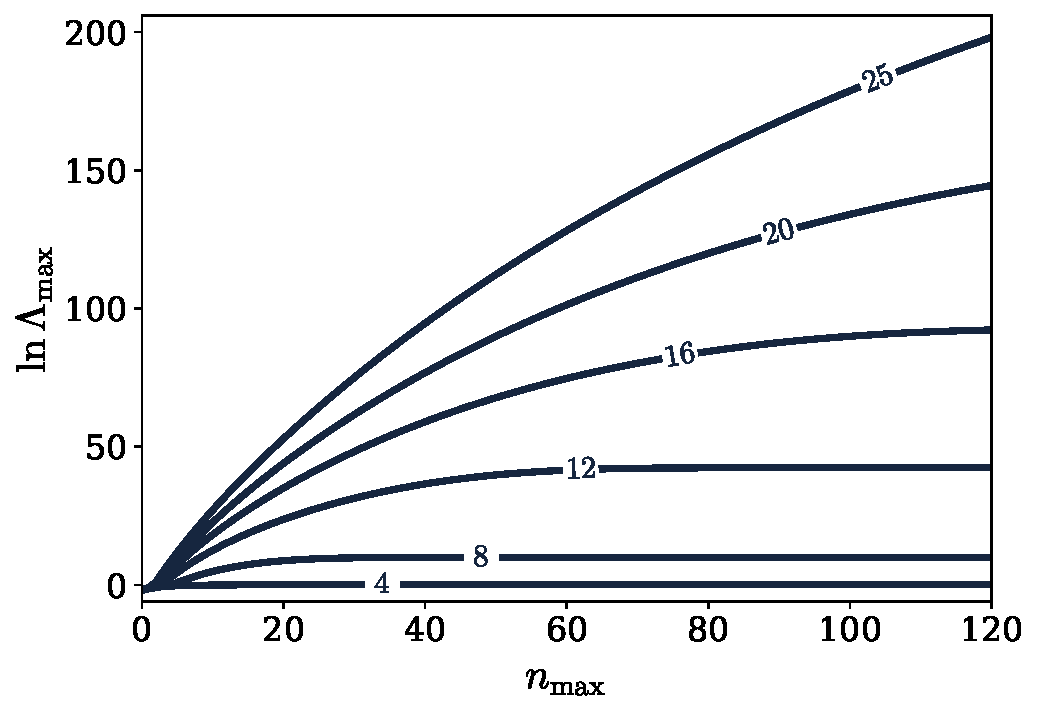
\includegraphics[width=\columnwidth]{lnlmax.pdf}
\caption{The truncated $\ln \Lambda$ against the truncation order
$n_{\max}$, at fixed matched filter SNRs (curves, labeled by
$\rho_{\rm mf}$), for one event whose distance sets the SNR. Each
curve rises with the order and saturates once $n_{\max}$ passes the
largest term of the series, at $n \simeq \rho_{\rm mf}^2 / 2$. For
example, $n_{\max} = 20$ statistics are ``good enough'' for every
signal up to $\rho_{\rm mf} \simeq 6$.}
\label{fig:lnlmax}
\end{figure}

\section{SGWB Search}
\label{sec:population}

We demonstrate the search on a simulated intermittent background. Binary black holes (BBHs) merge at the GWTC consistent rate density $R_0 = 30~{\rm Gpc^{-3}\,yr^{-1}}$, with a power law plus peak chirp mass model, and are injected into $3 \times 10^4$ segments of 4 s in the two LIGO detectors at the A+ design sensitivity. In total we simulate 111 days of data, which we divide into 20 chunks. The population model carries 4 free parameters, the rate density $R_0$ and the mass model $(\alpha, f_{\rm peak}, \mu)$. The full population and simulation configuration is given in Appendix~\ref{app:simpop}.

\begin{figure*}[!t]
\centering
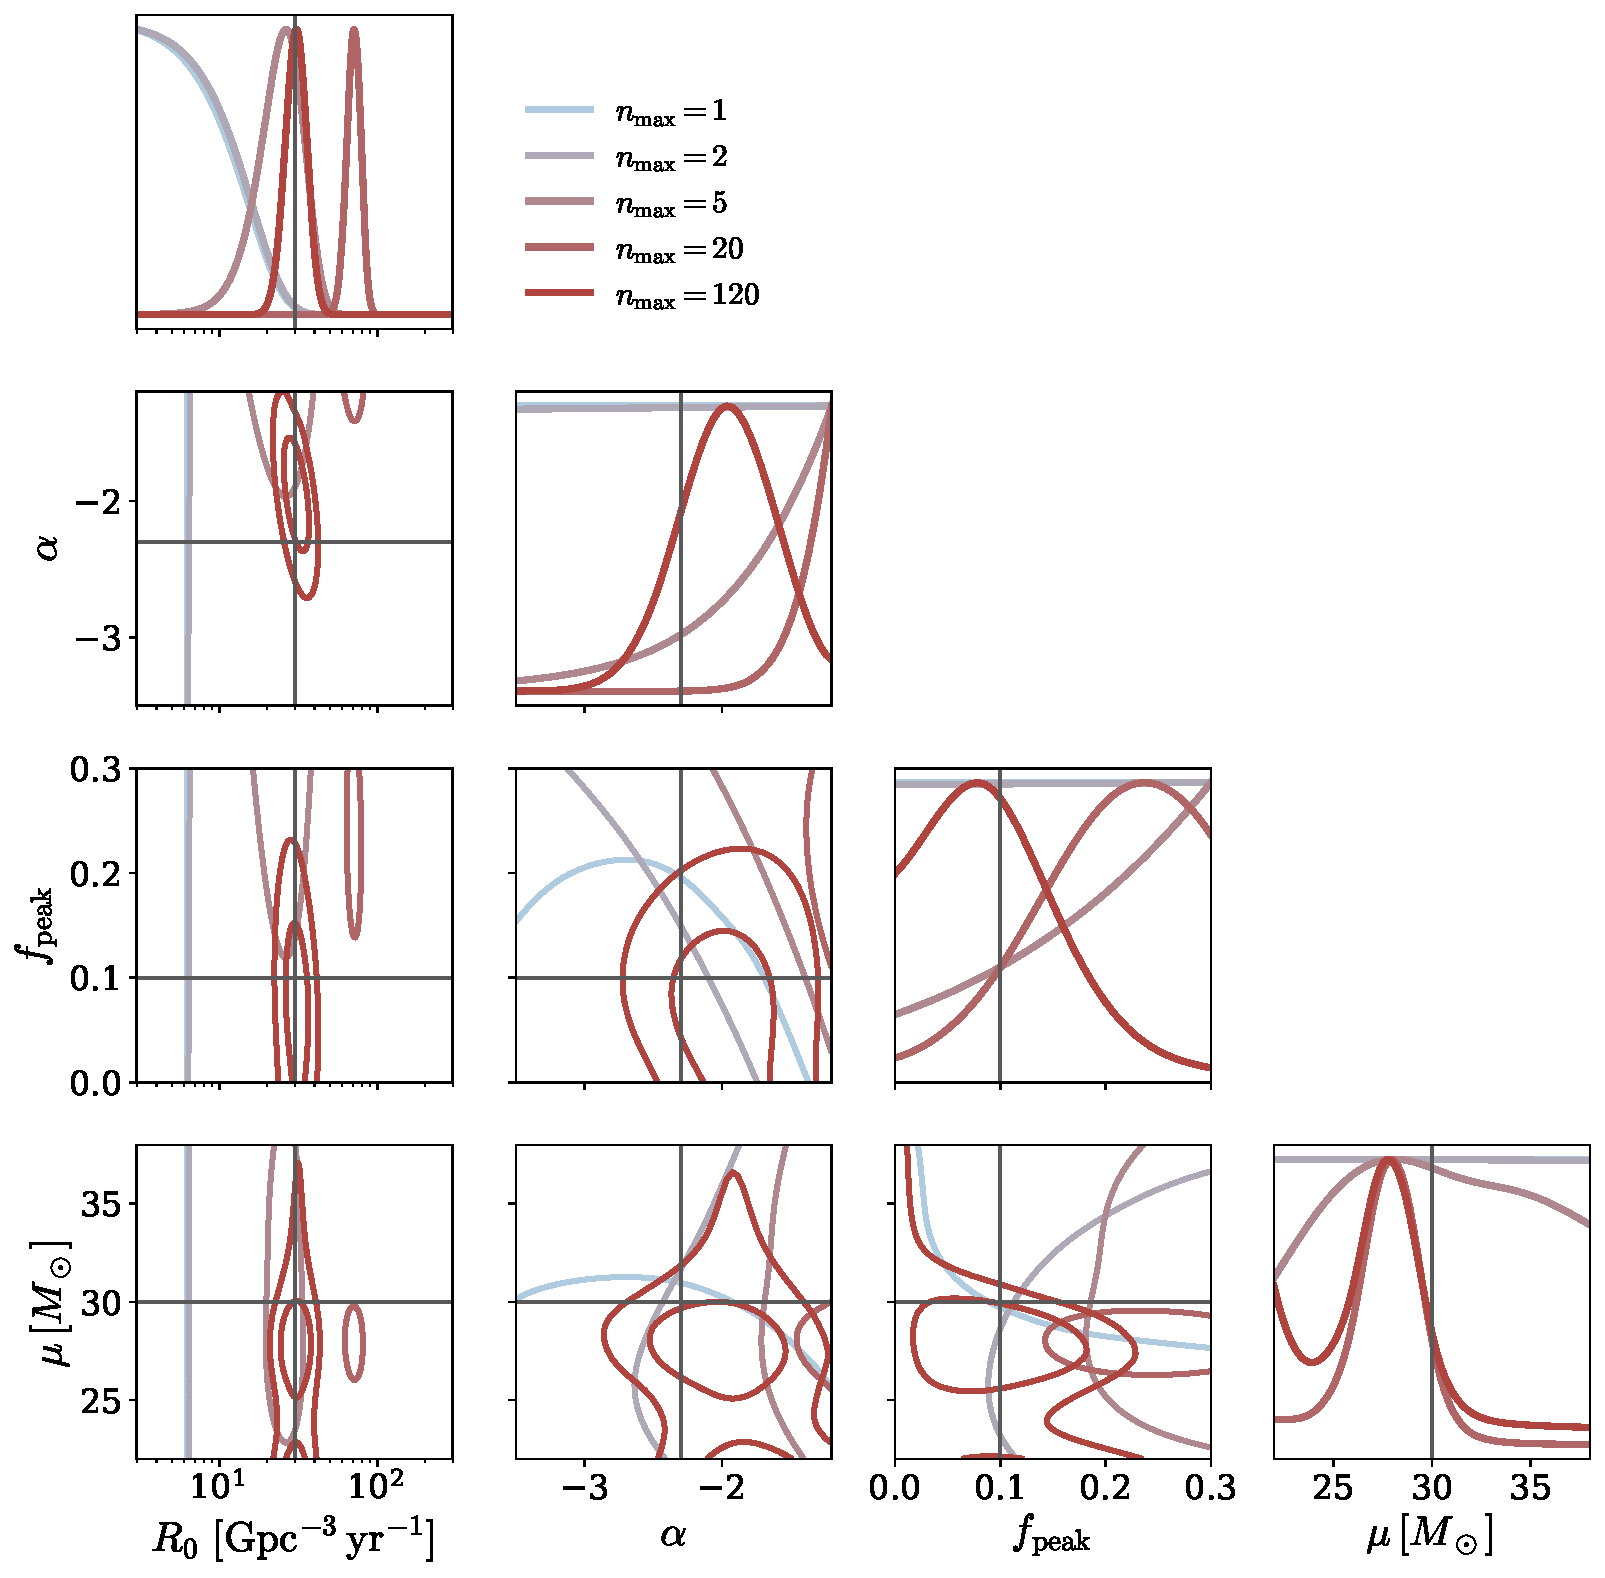
\includegraphics[width=0.57\textwidth]{sgwb_depths.pdf}\hfill
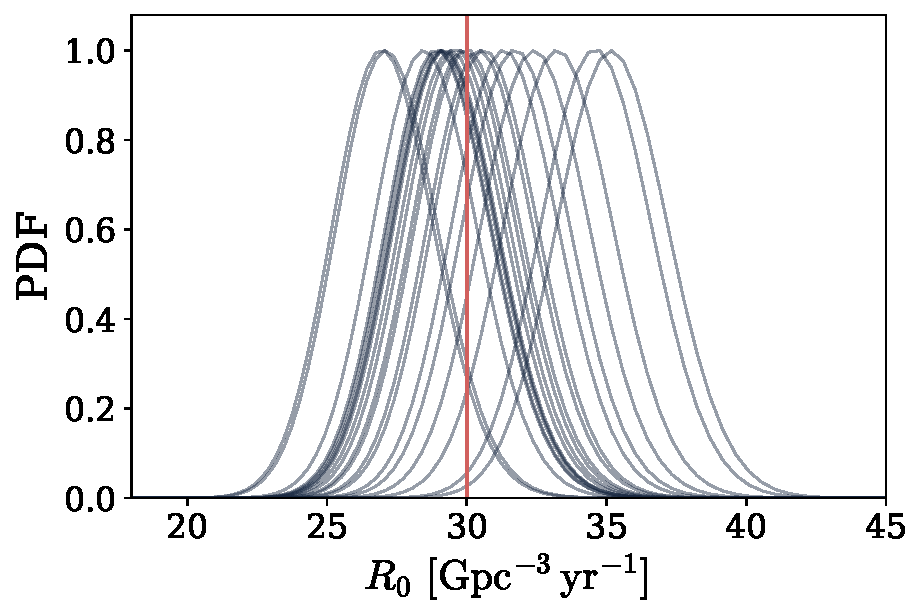
\includegraphics[width=0.41\textwidth]{r0_realizations.pdf}
\caption{Left, population posteriors at varying truncation orders
$n_{\max}$, on the main set. The truncations $n_{\max} = 1$ and 2
rail the rate to zero and the mass peak to the prior edge, the
recovery turns on at $n_{\max} = 5$, and the posterior saturates by
$n_{\max} = 20$. Grey lines mark the injected values, the red line
on the right the injected rate. Right, merger rate posteriors over
the 20 chunks at $n_{\max} = 120$, each peak normalized,
with the mass model held at the injection. The 90 percent
interval covers the injected rate in 17 of the 20.}
\label{fig:pop}
\end{figure*}

Each segment is evaluated once with the pipeline of
Sec.~\ref{sec:method}, on an intrinsic template grid specified in
Appendix~\ref{app:simpop}, producing a stored matrix
$\Lambda^\star_i(\vec\lambda_k)$ over the segments and the 1792
templates, evaluated once and reused by every fit below. The mass hyperparameters enter through the per segment
population statistic
\begin{equation}
\bar\Lambda^\star_i(\alpha, f_{\rm peak}, \mu)
= \sum_k w_k(\alpha, f_{\rm peak}, \mu)\,
\Lambda^\star_i(\vec\lambda_k),
\label{eq:lbar}
\end{equation}
with the weights $w_k$ of the population mass model, specified in
Appendix~\ref{app:simpop}, normalized to $\sum_k w_k = 1$ and
uniform over the mass ratio and spin axes.

The population statistic enters the mixture of Eq.~\eqref{eq:mixture}
in place of the likelihood ratio of the segment, and the log
likelihood of the whole chunk, relative to the noise only
model, is
\begin{equation}
\ln \frac{\mathcal{L}}{\mathcal{L}_0}
(R_0, \alpha, f_{\rm peak}, \mu)
= \sum_i \Big[ -\bar N
+ \ln\big( 1 + \bar N\, \bar\Lambda^\star_i \big) \Big],
\label{eq:popfit}
\end{equation}
with $\bar N = R_0 V T_{\rm seg}$ set by the rate density and the
volume $V$ of the distance prior. The posterior is a direct grid
evaluation over the 4 hyperparameters with flat priors, and the
detection statistic $\Delta \ln \mathcal{L}$ is the maximum of
Eq.~\eqref{eq:popfit} against the background free model
$R_0 \to 0$.

We first analyze one chunk at varying truncation orders, from
$n_{\max} = 1$ to 120, and the left panel of Fig.~\ref{fig:pop}
shows the posteriors of the 4 hyperparameters. At $n_{\max} = 1$ and 2,
quadratic and quartic in the data, the rate posterior collapses to zero
and the mass peak is pushed to the edge of its prior. The recovery turns
on at $n_{\max} = 5$, the posterior saturates by $n_{\max} = 20$,
and at the full order the joint posterior covers the injected values,
the rate at 23 to 38 ${\rm Gpc^{-3}\,yr^{-1}}$ at 90 percent
with the mass peak at $\mu = 27\,M_\odot$ against the injected 30,
while the noise only set drives the rate to zero. At
$n_{\max} = 120$ we then fit the rate on the 20 chunks
separately, to test the consistency of the recovery, with the
mass model held at the injection, and the right panel of
Fig.~\ref{fig:pop} shows the 20 posteriors.

\begin{figure*}[!t]
\centering
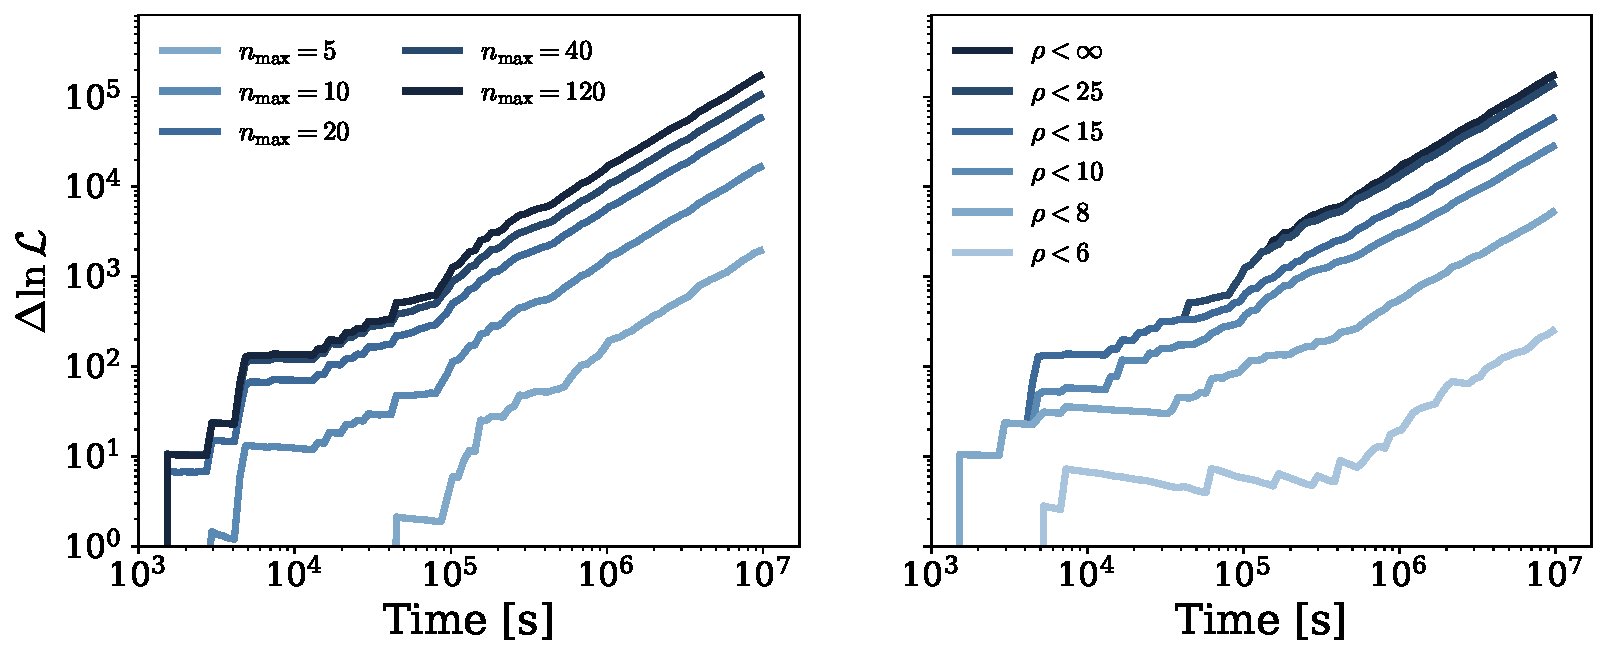
\includegraphics[width=\textwidth]{bf_vs_time_aplus.pdf}
\caption{The detection statistic against the observing time, the
mass model held at the injection and the rate profiled at every
checkpoint, on the 20 chunks combined into one
observation of 111 days. Left, the truncation orders, where
$n_{\max} = 1$ and 2 stay below one over the entire range and do
not enter the panel. Right, the full order $n_{\max} = 120$ with
every segment whose loudest event exceeds the matched filter SNR
cut removed, over a ladder of cuts.}
\label{fig:bftime}
\end{figure*}

Figure~\ref{fig:bftime} accumulates the detection statistic over
the observing time, on the 20 chunks combined into one
observation of 111 days. At every checkpoint the sum of
Eq.~\eqref{eq:popfit} over the segments observed so far is
profiled over the rate. In the left panel the truncation orders
$n_{\max} = 1$ and 2 never detect, the information turns on at
$n_{\max} = 5$, and the full order reaches
$\Delta \ln \mathcal{L} = 1.7 \times 10^{5}$ over the full
observation. To see how much of the contribution is coming from which
subthreshold events, in the right panel every segment whose
loudest event exceeds a matched filter SNR cut is removed before
the accumulation. With every event below $\rho = 8$ the search
passes a profile log likelihood ratio of
$\Delta \ln \mathcal{L} = 8$ within
half an hour of data, and with every event below $\rho = 6$
within 5 days. This is the profile statistic of
Eq.~\eqref{eq:popfit}, not a Bayes factor, and we do not read it
as posterior odds.


We also test the effect of the segment duration in
Appendix~\ref{app:tseg}, lengthening the segments to 8, 32, and
192 s, for which the single event condition $\bar N \ll 1$
breaks down at the larger durations. The overlapping events, which
the mixture does not model, pull the recovered rate down
monotonically with the duration, to 26 at 8 s, to 18 at 32 s, and
to 7 at 192 s against the injected 30, while the mass peak stays
at 27 to 33 $M_\odot$. The overlap therefore biases the rate but
not the shape of the mass model.

Each template evaluation takes a few milliseconds, and the full run
of the demonstration completes in under an hour on a computing
cluster. On the same data the posteriors of individual segments match
the \texttt{bilby} sampler \cite{bilby} at more than an order of
magnitude lower cost, and the cost ratio grows with the SNR, as there is no run time cost for the larger truncation orders that louder signals require.

\FloatBarrier

\section{Conclusion}
\label{sec:conclusion}

We asked when individually resolvable signals become a stochastic
gravitational wave background, and the answer is a continuous
family rather than a threshold. The cross correlation statistic
is the first order of the extrinsic marginalization of a compact
binary signal in two detectors, the higher orders collect into
generalized overlap reduction functions contracted with cross
moments of the matched filter outputs, and the untruncated series
is the fully marginalized event likelihood. The transition is
quantified. The standard overlap reduction function is the
optimal weight only below a matched filter SNR of about 0.1, a
signal at SNR $\rho_{\rm mf}$ requires
$n_{\max} \simeq \rho_{\rm mf}^2 / 2$ statistics, and $O(100)$
statistics carry a reliable search of the full subthreshold
population. The tables are computed once, the truncation is
controlled with an analytic normalization, and the evaluation
costs milliseconds per template, so the search runs at observing
run scale.

On single events the series reproduces the exact marginalized
likelihood with unbiased posteriors over 592 injections. On a
simulated background at the A+ sensitivity, 111 days of data
recover the merger rate at 23 to 38 ${\rm Gpc^{-3}\,yr^{-1}}$
against the injected 30, with the mass peak at 27 $M_\odot$
against the injected 30, and the detection stands within 5 days
of data after the removal of every event above matched filter
SNR 6, carried by the subthreshold population alone.

The construction is not tied to the terrestrial network. Any
search built on the cross correlation of detector pairs, with an
overlap reduction function as its geometric weight, admits the
same expansion, and a pulsar timing array, where the Hellings
Downs curve plays this role, is a natural next target. The
overlapping events of longer segments sit beyond the single event
mixture here, and the companion paper holds the full Poisson
series that carries them.

\begin{acknowledgments}
Computations used the Minnesota Supercomputing Institute.
\end{acknowledgments}

\bibliography{refs}

\clearpage
\onecolumngrid
\begin{center}
{\large\bf Supplemental Material}
\end{center}
\appendix

\section{Mode Counting}
\label{app:modes}

To get an intuition on how many statistics a single event likelihood
must carry at a given SNR, we perform a simple one
parameter experiment. Here we fix every extrinsic parameter of the
binary except the arrival time $t_c$, inject a signal at a true
arrival time, and evaluate a template at a filter time $t_f$, with
the log likelihood ratio
\begin{equation}
\ln \Lambda(t_f, t_c) = 2\,\mathrm{Re}\,\langle d \,|\, h(t_f) \rangle
- \langle h(t_f) \,|\, h(t_f) \rangle,
\label{eq:tcllr}
\end{equation}
with the data $d = h(t_c) + n$ carrying the signal at the true time
$t_c$ and $n$ the noise. The template norm
$\langle h | h \rangle = \rho^2$ does not depend on time, so the shape
is set by the matched filter $\langle d | h(t_f) \rangle$, which peaks
at $t_f = t_c$. Scanning a grid of true and filter times builds the
matrix $\ln \Lambda(t_f, t_c)$ of Fig.~\ref{fig:tcmatrix}, which
sharpens from a broad ridge to a diagonal as the SNR
grows.

\begin{figure*}[htb]
\centering
\centering
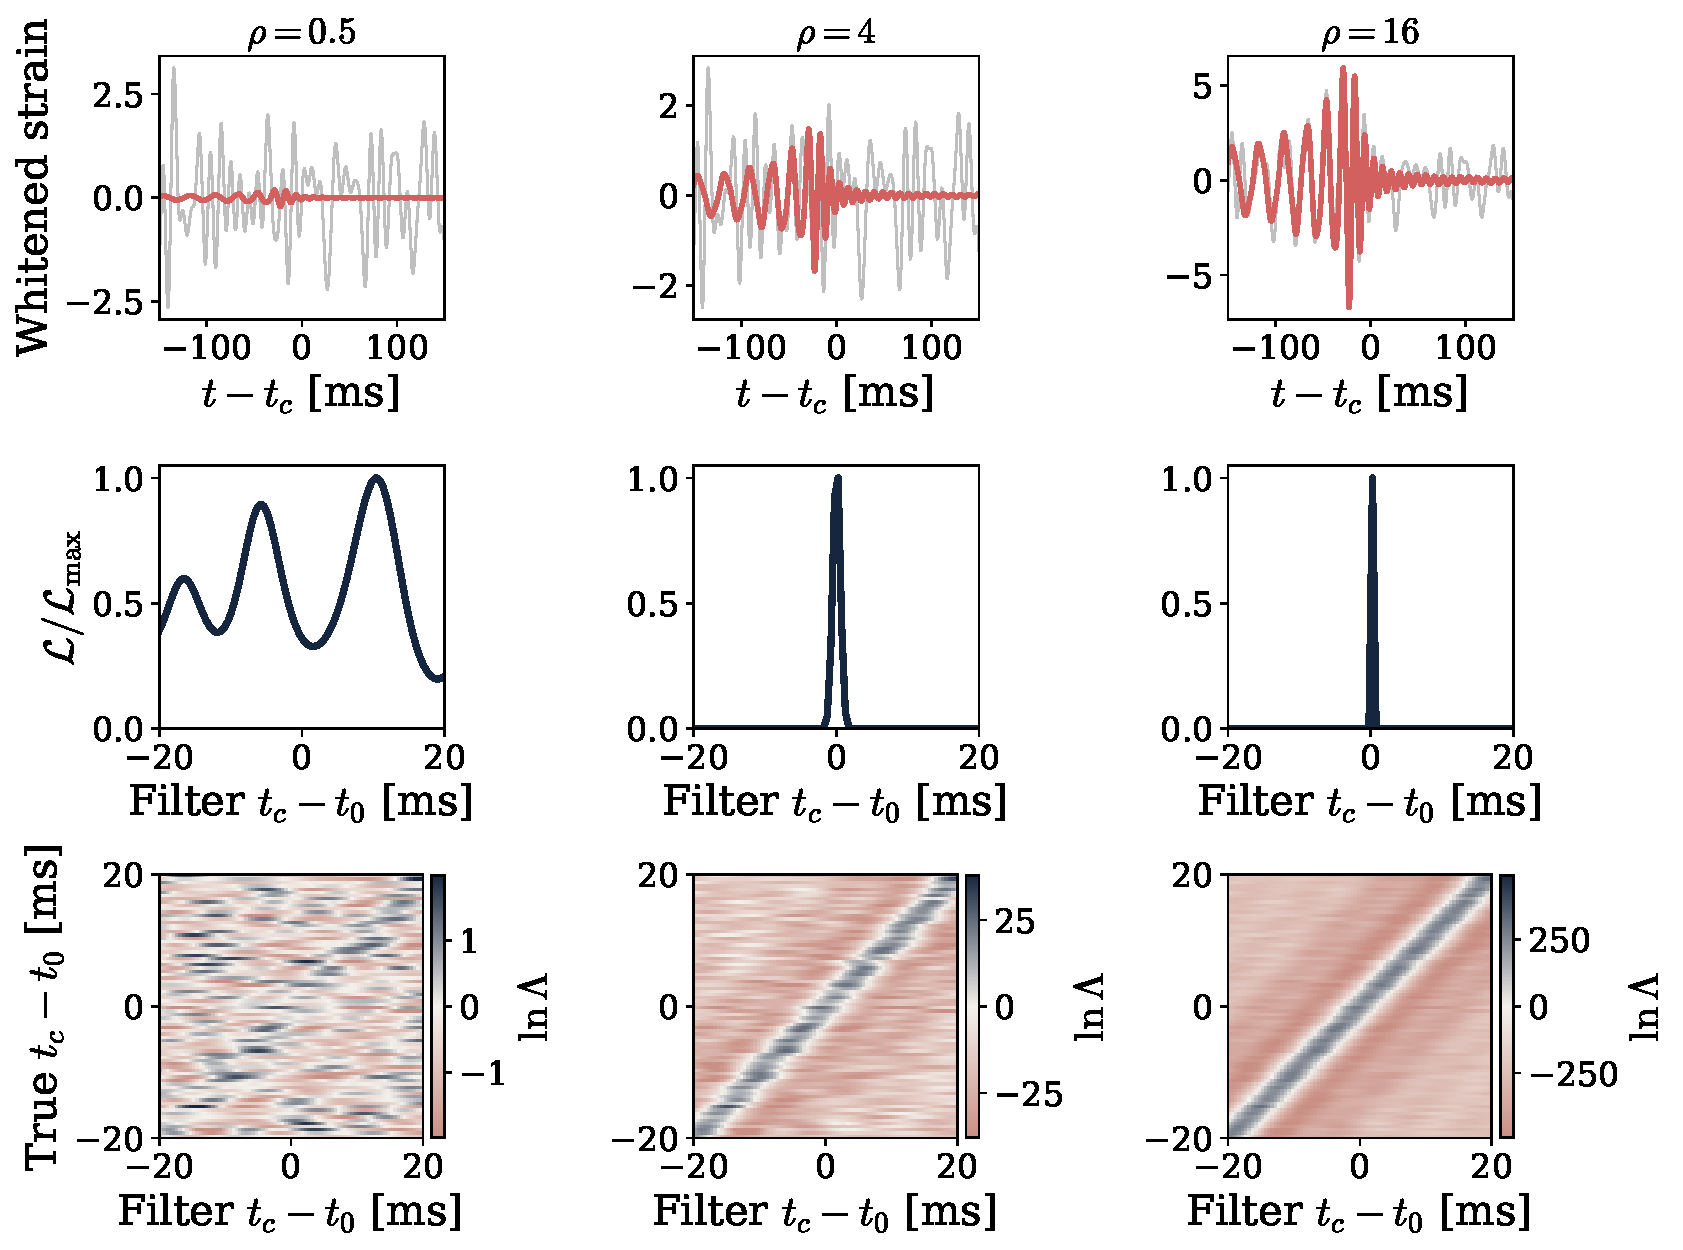
\includegraphics[width=0.7\textwidth]{tc_matrix.pdf}
\caption{The single parameter experiment, everything frozen except the arrival time $t_c$, at 3 SNRs. Top, whitened data (grey) with the sliding matched filter (red). Middle, the likelihood in the filter time, which narrows from a broad maximum to a sharp peak. Bottom, the log likelihood ratio over the plane of true and filter arrival time, whose peak sharpens from broad to narrow. The number of modes is set not by this matrix but by the noise covariance of the likelihood ratio, Eq.~\eqref{eq:kernel}, which passes from one dominant mode to the full rank of the matched filter.}
\label{fig:tcmatrix}
\end{figure*}

The number of terms the event needs is the effective rank of the noise
covariance of the likelihood ratio $\Lambda = e^{\ln\Lambda}$ across
the filter times,
\begin{equation}
K_{jk} = \mathbb{E}_{\rm noise}\!\big[(\Lambda_j - 1)(\Lambda_k - 1)\big],
\qquad \Lambda_j = \Lambda(t_{f,j}, t_c),
\label{eq:kernel}
\end{equation}
the average taken over noise at fixed true time. Since the
injected signal is held fixed, $K_{jk}$ is not the centered
covariance of $\Lambda$; we use it only as a mode counting
diagnostic, and its eigenspectrum measures how the variation of
the likelihood ratio across the filter times spreads over the
directions. The log likelihood
ratio of Eq.~\eqref{eq:tcllr} is linear in the noise, so this average
is carried out in closed form and $K_{jk}$ reduces to the overlaps of
the filter templates. At low SNR
the filter cannot localize the signal, $\Lambda$ is nearly constant over the
filter time, and $K$ has one dominant mode, so a single summary
statistic, the average of the likelihood ratio over the filter times,
carries the estimate. At high SNR only the matching filter responds,
$\Lambda$ concentrates on the diagonal, and $K$ approaches the full
rank of the matched filter.

We then repeat the experiment for the overall phase $\varphi_0$
alone, and for the joint marginalization over the 5 extrinsic
parameters, the sky direction, the inclination, the polarization, the
phase and the arrival time. The single parameter cases scan a dense
one dimensional grid of filter values. A lattice over 5 parameters
is not affordable, so the joint case draws $2 \times 10^4$
configurations from the extrinsic prior, the sky uniform on the
sphere, the inclination cosine and the polarization uniform, the
phase uniform, and the arrival time uniform in a $\pm 25$ ms window,
and builds Eq.~\eqref{eq:kernel} on these draws. The normalized
eigenspectrum of $K$ flattens from one mode into many as the SNR
grows (Fig.~\ref{fig:svd}), the mode count rising into the hundreds
for a single parameter and the thousands for the joint
marginalization. For the subthreshold signals of interest, where the
SNR is low, of order a hundred terms suffice, and the series of
Eq.~\eqref{eq:master} carries them all at a cost independent of the
order.

\begin{figure*}[htb]
\centering
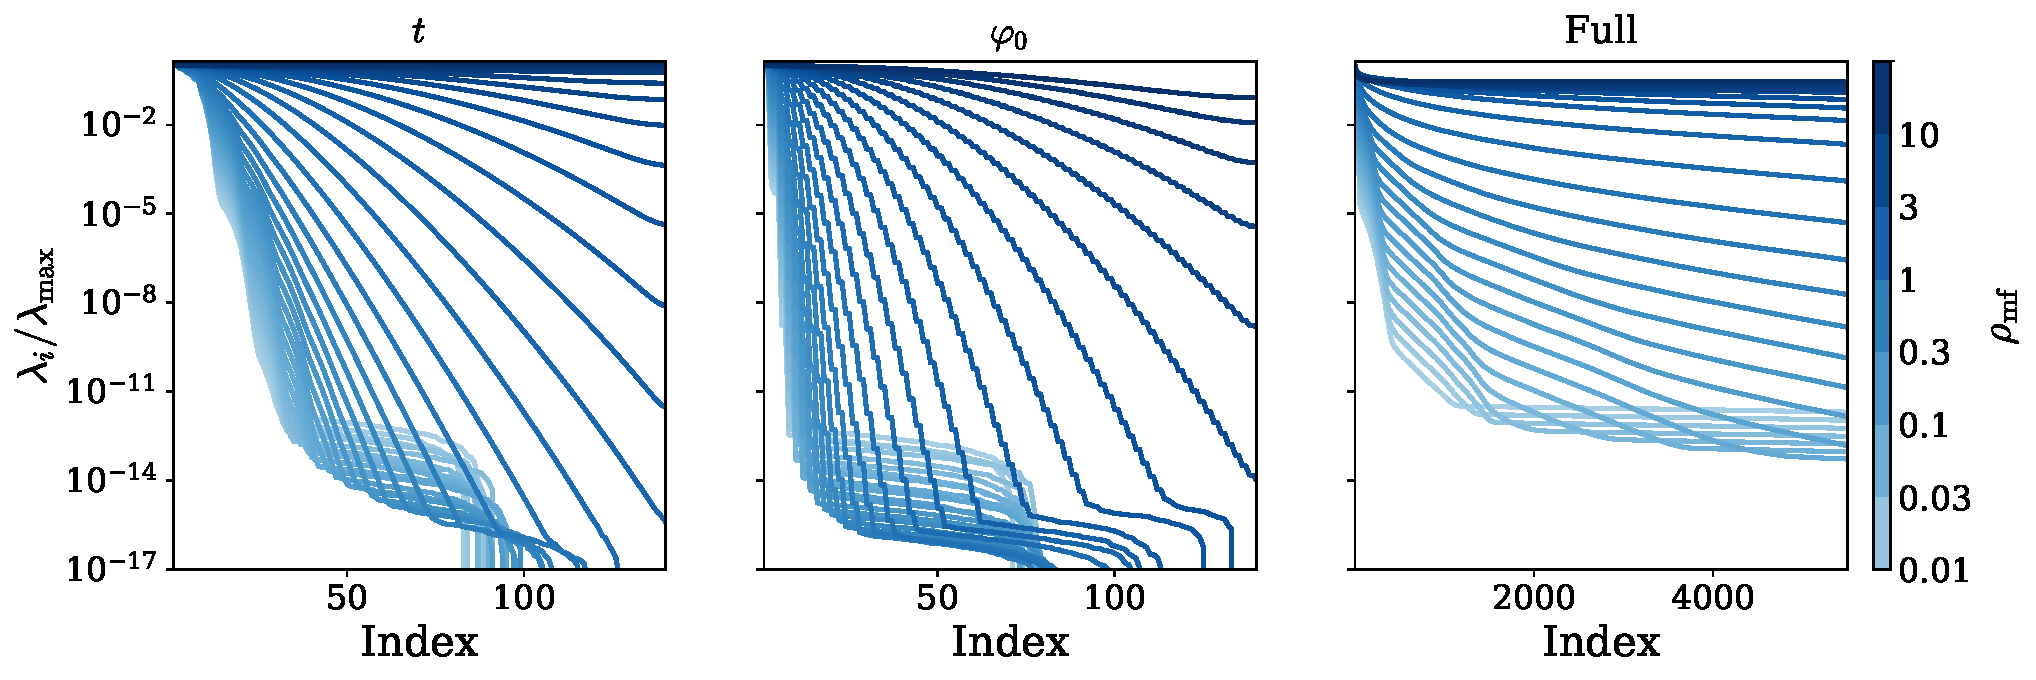
\includegraphics[width=0.75\textwidth]{svd_modes.pdf}
\caption{Normalized eigenvalue spectra of the noise covariance of the single event likelihood ratio, Eq.~\eqref{eq:kernel}, as a function of the SNR, for the marginalization over the arrival time alone, the coalescence phase alone, and the joint marginalization over the sky direction, inclination, polarization, coalescence phase and arrival time.}
\label{fig:svd}
\end{figure*}

\section{Construction of the Tables}
\label{app:construction}

We start by evaluating the distance moment $M_n(A)$ of
Eq.~\eqref{eq:W}. For the Euclidean prior
$p(y) = 3\, y_{\min}^3\, y^{-4}$ on $y > y_{\min}$ it reads
\begin{equation}
M_n(A) = \int_{y_{\min}}^{\infty} dy\, p(y)\, y^{2n} e^{-y^2 A},
\label{eq:Mndef}
\end{equation}
and the substitution $t = y^2 A$ evaluates it to the upper
incomplete gamma function \cite{DLMF},
\begin{equation}
M_n(A) = \frac{3}{2}\, y_{\min}^3\, A^{\frac{3-2n}{2}}\,
\Gamma\!\left( \frac{2n-3}{2},\, y_{\min}^2 A \right).
\label{eq:Mn}
\end{equation}
The bare moments of the prior are formally divergent. The uniform in
volume prior falls only as $y^{-4}$, so
$\int dy\, p(y)\, y^{2n} \sim \int dy\, y^{2n-4}$ grows without bound
at the loud end for every $n \geq 2$, where arbitrarily close sources
carry arbitrarily large amplitudes. But $M_n(A)$ is finite due to the
damping $e^{-y^2 A}$, the template norm term of the exponent of
Eq.~\eqref{eq:marg}, with $A = u_1 |R_1|^2 + u_2 |R_2|^2$ set by the
template powers and the responses. The likelihood itself cuts the
loud tail at $y \simeq 1/\sqrt{A}$.
Because the cut depends on the orientation through $A$, the table
cannot be split into a distance factor times a geometry factor, and
$M_n(A)$ must sit inside the orientation average.

The table is the discretized orientation average of
Eq.~\eqref{eq:W}. With the sky on a HEALPix grid of $N_{\rm pix}$
pixels, the polarization on a uniform grid of $n_\psi$ angles, and the
inclination cosine on a Gauss Legendre grid of $n_\chi$ points with
weights $w_\chi$,
\begin{equation}
W^{(n)}_{ab}(\tau_m, u_1, u_2) = \frac{1}{N_{\rm pix}\, n_\psi}
\sum_{\rm pix} \sum_{\psi} \sum_{\chi} \frac{w_\chi}{2}\,
M_n(A)\, R_1^a \bar R_1^b R_2^{n-a} \bar R_2^{n-b}\,
\Delta_m\!\big(\hat n \cdot \Delta \vec x / c\big).
\label{eq:Wdisc}
\end{equation}
We recall from Eqs.~\eqref{eq:zu} and \eqref{eq:ZA} that
$R_I = \tfrac{1+\chi^2}{2} F^I_+ + i \chi F^I_\times$ is the
response, $u_I = \sum_\nu a_\nu^2 / \sigma^2_{I,\nu}$ is the
template power, and $A = |R_1|^2 u_1 + |R_2|^2 u_2$, so the table
depends on the delay through the pixel geometry and on the template
powers through the damping. The function $\Delta_m(\tau)$ is the discretized delta function of
Eq.~\eqref{eq:W},
\begin{equation}
\Delta_m(\tau) = \max\!\big( 0,\, 1 - |\tau - \tau_m| / \delta\tau
\big),
\label{eq:deposit}
\end{equation}
which spreads the delay of each pixel linearly over the two
neighboring points of a uniform delay grid with spacing
$\delta\tau$. A Kronecker delta onto the nearest point would shift
every pixel delay by up to $\delta\tau/2$ and make the table noisy
at the grid scale. The grid spans the light travel time of the
baseline, $|\tau| \leq |\Delta \vec x|/c \approx 10$ ms. At $n_{\max} = 120$ the grids have $3072$ sky pixels, $243$
polarization angles, and $123$ inclination points. The
symmetry $\chi \to -\chi$ of the inclination prior makes the tables
real and symmetric under $(a, b)$ exchange, so only $b \leq a$ is
kept.

The sky resolution sets the accuracy of $W^{(n)}_{ab}(\tau)$,
because the delay distribution inherits the pixel scale. At $N_{\rm side} = 8$
the table oscillates at the pixel scale and biases $\ln \Lambda$ by
about $0.1$ on injected data, at $N_{\rm side} = 16$ the bias is
smaller than $0.007$ in $\ln \Lambda$, the residual of the direct
check at the end of this appendix, and $N_{\rm side} = 32$ and $128$
coincide
(Fig.~\ref{fig:Wnside}). The analysis uses $N_{\rm side} = 16$.

\begin{figure}[htb]
\centering
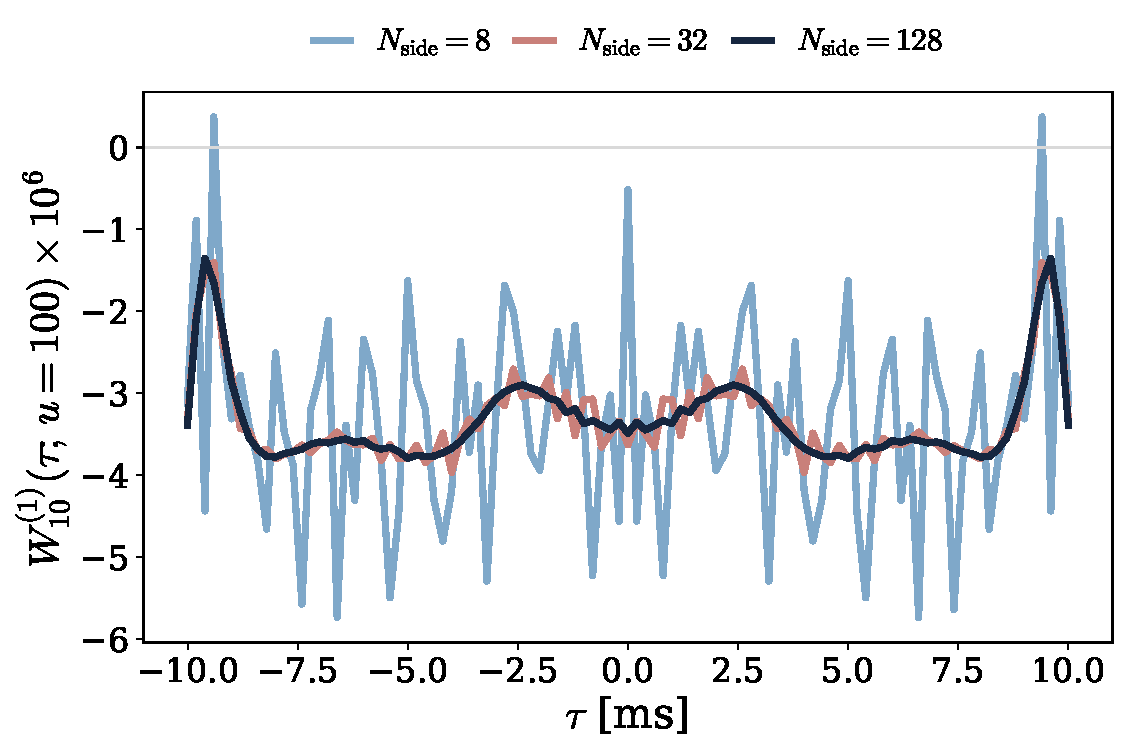
\includegraphics[width=0.45\textwidth]{W_nside.pdf}
\caption{Sky quadrature convergence of one geometric table with
the HEALPix resolution. At $N_{\rm side} = 8$ the curve oscillates
at the pixel scale, while $N_{\rm side} = 32$ and $128$
coincide. The analysis uses $N_{\rm side} = 16$.}
\label{fig:Wnside}
\end{figure}

We precompute the tables on a one dimensional grid of template
powers $u_{\rm grid}$. We assumed equal noise in the two detectors,
so the two powers coincide, $u_1 = u_2 = u$. A template in general
falls between the grid points. When a segment arrives we compute
from the data the integrals $T^{(n)}_{ab}(\tau)$ of
Eq.~\eqref{eq:T} and the template power $u$ of Eq.~\eqref{eq:zu},
and we contract $T^{(n)}$ with the stored $W^{(n)}$ of
Eq.~\eqref{eq:Wdisc}. The stored tables exist only at the grid
powers, so we first rescale the data integrals to the nearest grid
power, $T^{(n)} \to (u_{\rm grid}/u)^n\, T^{(n)}$. The rescaling is
exact, because $u$ and the distance amplitude $y$ enter
Eq.~\eqref{eq:marg} only through the product $u y^2$, so lowering
$u$ to $u_{\rm grid}$ and raising $y^2$ by the same factor leaves
the likelihood unchanged. The one quantity that does not follow is
the lower limit of the distance prior, which moves from $y_{\min}$
to $y_{\min} \sqrt{u/u_{\rm grid}}$. To increase the accuracy we
evaluate at the two grid points around $u$ and interpolate linearly
in $\ln u$, and the residual stays smaller than $0.05$ in
$\ln \Lambda$ across the grid spacing.

The complete construction is checked against a direct evaluation of
Eq.~\eqref{eq:marg} with the exact Bessel function. On one injected
event the two differ by $0.106$ in $\ln \Lambda$, of which $0.099$
is the rounding of the arrival time to the sample grid on the data
side. Once the rounding is matched the remaining difference is
$0.007$, negligible against the statistical scales of the analysis.

\section{Truncation Errors}
\label{app:norm}

A likelihood ratio has unit mean under noise, because the signal
likelihood in its numerator is normalized,
\begin{equation}
\mathbb{E}_{\rm noise}[\Lambda] = \int \mathcal{D}d\;
\mathcal{L}_n(d)\, \frac{\mathcal{L}_s(d)}{\mathcal{L}_n(d)}
= \int \mathcal{D}d\; \mathcal{L}_s(d) = 1 .
\label{eq:unitmean}
\end{equation}
In our construction we terminate the series at the order $n_{\max}$,
therefore this condition is not automatically satisfied.

\begin{figure*}[htb]
\begin{minipage}[t]{0.54\textwidth}
\centering
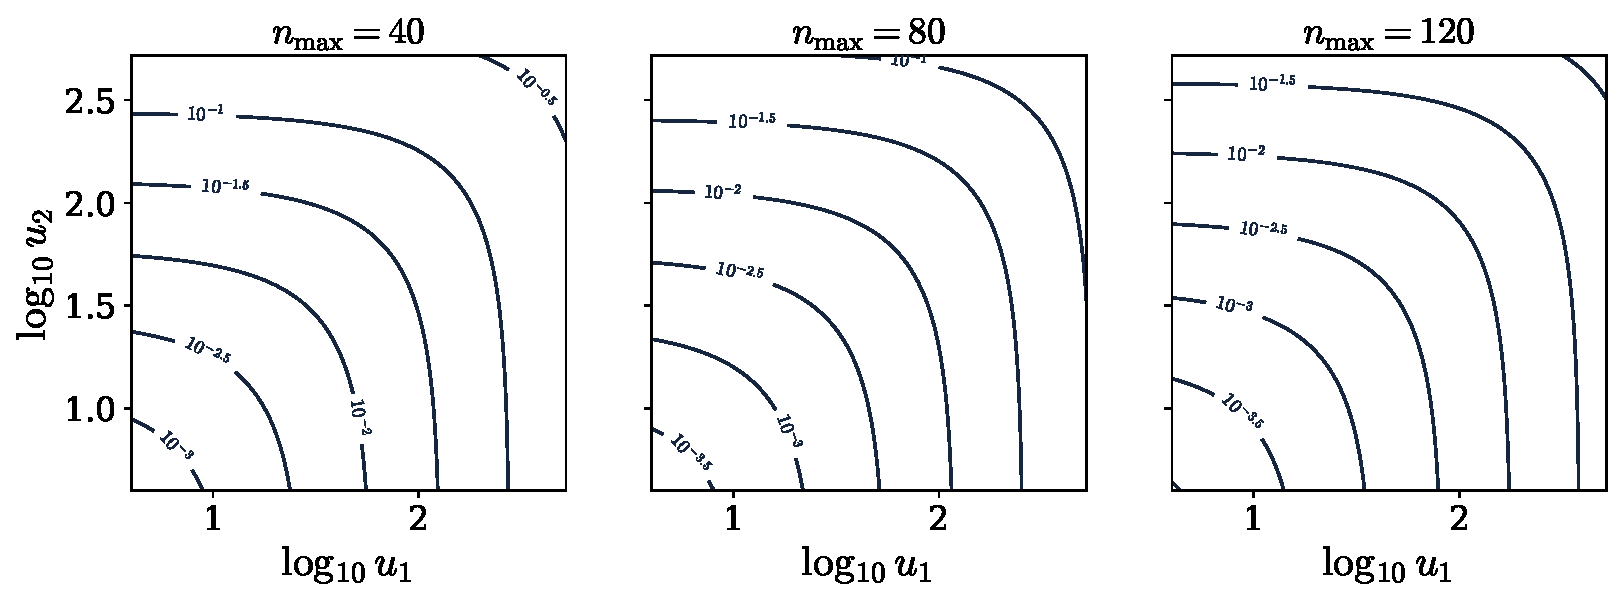
\includegraphics[width=\linewidth]{eps_u1u2.pdf}
\caption{The truncation normalization $\epsilon_{n_{\max}}(u_1, u_2)$ of
Eq.~\eqref{eq:eps} over the two detector template powers, at 3
truncation orders. It depends on the powers only through
$A = u_1 |R_1|^2 + u_2 |R_2|^2$, and identical detector noise
samples the plane along $u_1 = u_2$. It is a $10^{-3}$ level correction over most of
the plane and rises toward the loud edge, where the unbounded distance
prior keeps a nonzero weight.}
\label{fig:eps}
\end{minipage}\hfill
\begin{minipage}[t]{0.42\textwidth}
\centering
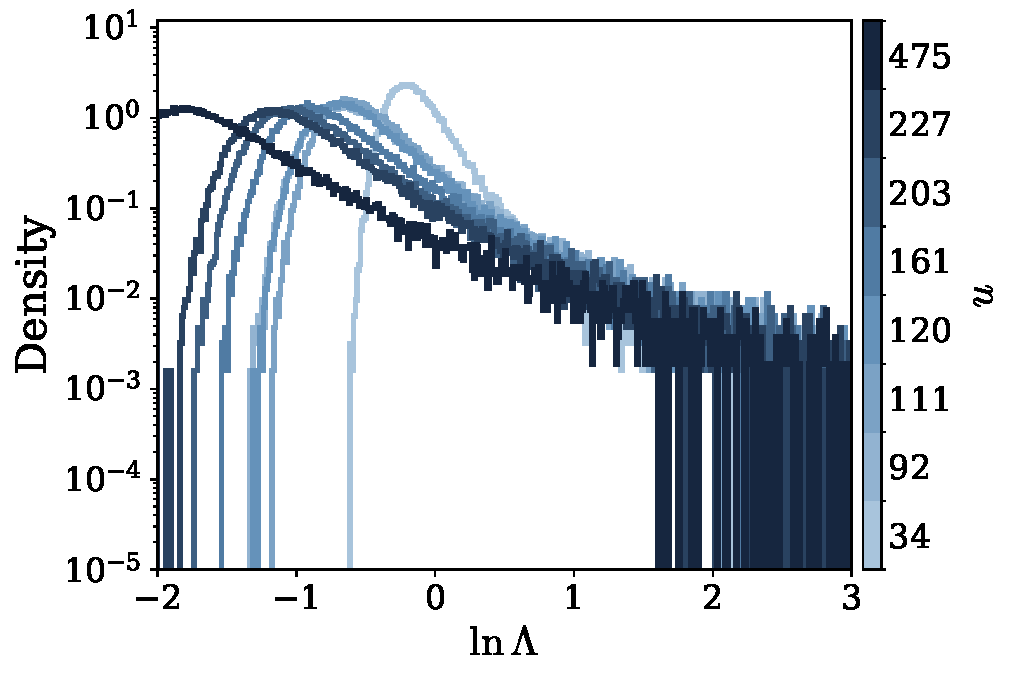
\includegraphics[width=\linewidth]{noise_hist.pdf}
\caption{Noise only distributions of $\ln \Lambda$ at
$n_{\max} = 120$ for 8 template power values $u$. The bulk
moves to negative values as $u$ grows while a heavy right tail
persists, so a finite sample mean lies below the unit
expectation. The distribution is unchanged at $n_{\max} = 40$
and 80.}
\label{fig:noise}
\end{minipage}
\end{figure*}

The population fit of Eq.~\eqref{eq:popfit} sums
$\sum_i \big[ -\bar N + \ln(1 + \bar N \bar\Lambda_i) \big]$
over the segments. On a noise only segment the derivative in
$\bar N$ has mean $\mathbb{E}[\bar\Lambda] - 1$. With the exact
statistic this mean is zero and noise segments carry no preference
on the rate. Without the normalization it becomes negative, every
noise segment pulls the rate toward zero, and the pulls add up over
the millions of segments of a search.

One could restore the normalization by simulating a large set of
noise only segments, evaluating them for every template, and
dividing by the sample mean. However, as we show in Fig.~\ref{fig:noise},
the noise distribution of $\ln \Lambda$ is heavy tailed, the bulk
moves to negative values as the template power grows while a rare
right tail carries the mean, so a finite sample mean lies below the
true mean, and the division biases the recovered rate high by a
factor of a few. Therefore we compute the normalization
analytically.

At fixed extrinsic parameters and distance the noise enters through
the coherent combination of Eq.~\eqref{eq:ZA},
$Z = R_1 z_1(t + \tau) + R_2 z_2(t)$, which under noise is a
complex Gaussian with variance $\langle |Z|^2 \rangle = A$, so its
even moments are
\begin{equation}
\mathbb{E}_{\rm noise}\big[ |Z|^{2n} \big] = n!\, A^n .
\label{eq:noisemom}
\end{equation}
The $n$th term of the expansion of Eq.~\eqref{eq:taylor} enters
Eq.~\eqref{eq:bessel} as $(y |Z|)^{2n} / (n!)^2\, e^{-y^2 A}$, and
by Eq.~\eqref{eq:noisemom} its noise mean at fixed
$(\vec\theta, y)$ is
\begin{equation}
\frac{y^{2n}\, n!\, A^n}{(n!)^2}\, e^{-y^2 A}
= e^{-y^2 A}\, \frac{(y^2 A)^n}{n!},
\label{eq:poisweight}
\end{equation}
which is the Poisson weight of mean $y^2 A \simeq \rho_{\rm mf}^2/2$.
The weights sum to one over all $n$, which recovers
Eq.~\eqref{eq:unitmean}. Summing them only up to $n_{\max}$ and
marginalizing over the orientation and the distance gives the noise
mean of the truncated statistic,
\begin{equation}
\mathbb{E}_{\rm noise}[\Lambda] = \big\langle
P[\,\mathrm{Pois}(A y^2) \leq n_{\max}\,]
\big\rangle_{\vec\theta, y} = 1 - \epsilon_{n_{\max}}(\vec\lambda),
\label{eq:truncmean}
\end{equation}
smaller than one by the averaged Poisson tail
\begin{equation}
\epsilon_{n_{\max}}(\vec\lambda) = \Big\langle \int_0^\infty dy\, p(y)\,
P[\,\mathrm{Pois}(A y^2) > n_{\max}\,] \Big\rangle_{\hat n, \psi, \chi},
\label{eq:eps}
\end{equation}
with $P[\mathrm{Pois}(x) > n_{\max}]$ the regularized lower incomplete
gamma function $\gamma(n_{\max}+1, x)/n_{\max}!$ \cite{DLMF} and
$p(y)$ the distance prior. We evaluate Eq.~\eqref{eq:eps} with the
same orientation grids as Eq.~\eqref{eq:Wdisc} and a logarithmic $y$
grid, and tabulate it once over the template powers.

The corrected statistic is
\begin{equation}
\Lambda^\star = \Lambda + \epsilon_{n_{\max}}(\vec\lambda),
\label{eq:lamstar}
\end{equation}
and the two objects separate cleanly. $\Lambda$ is the truncated
series, positive, below the untruncated statistic term by term, and
its noise mean is smaller than one by exactly $\epsilon_{n_{\max}}$.
$\epsilon_{n_{\max}}$ is nonnegative, carries no data,
depends on the template only through the powers $(u_1, u_2)$, and
restores $\mathbb{E}_{\rm noise}[\Lambda^\star] = 1$ at every
truncation order. Since the truncation error is positive with mean
$\epsilon_{n_{\max}}$ under noise, the correction also bounds the mean
error of the truncated statistic. The tail is negligible while the
largest term of the series stays below $n_{\max}$, growing only as
$\rho_{\rm mf}$ approaches $\sqrt{2 n_{\max}} \approx 15.5$, so over
the subthreshold range it stays below the percent level.

We test this normalization on $1.2 \times 10^5$ noise only
segments, evaluated over the full template bank. At the lowest
template powers the sample mean of $\Lambda^\star$ is $0.993$. At
the highest powers it drops to $0.52$ although the exact mean is
one, which is the finite sample effect of the heavy tail of
Fig.~\ref{fig:noise}.

Figure~\ref{fig:eps} shows $\epsilon_{n_{\max}}(u_1, u_2)$ over the two
detector template powers, on which it depends only through
$A = u_1 |R_1|^2 + u_2 |R_2|^2$. With equal detector noise every
template has $u_1 = u_2$, so the analysis samples the plane along that
line. The rest of the plane is the unequal noise generalization. Its
median over the analysis range is $1 \times 10^{-2}$ at
$n_{\max} = 120$, but because the distance prior
$p(y) \propto y^{-4}$ gives arbitrarily loud sources a nonzero weight,
the maximum at the loud edge is larger, $0.12$ at $n_{\max} = 120$ and
$0.39$ at $n_{\max} = 40$.
The single condition $\rho_{\rm mf} < \sqrt{2 n_{\max}}$ is therefore not
a global condition, and the loud edge is controlled instead by
restricting the analysis prior to the domain where $\epsilon_{n_{\max}}$
is small.

\section{Validation on Single Events}
\label{sec:validation}

The truncation order $n_{\max}$ controls how well the series reproduces the full likelihood. In Appendix~\ref{app:modes} we demonstrate a simple case, with every parameter of the binary fixed except the arrival time, which shows how the information carried by the likelihood spreads from a single statistic at low SNR over hundreds of statistics as the SNR grows. This motivates us to also investigate directly how large a truncation order is needed in the full analysis to achieve the exact marginalized likelihood over the range of interest. The run time cost does not depend on $n_{\max}$, so the order is set by accuracy alone.




We evaluate the method of Eq.~\eqref{eq:master} on individual events for a range of $n_{\max}$ and SNR. We simulate one CBC event in two detectors at equal noise, at a representative sky position, orientation, and intrinsic parameters, and vary its distance to set the SNR and the truncation order. Figure~\ref{fig:corner} shows exact grid posteriors of one event, on the left across a range of SNR at fixed $n_{\max} = 40$, and on the right at a matched filter SNR of 25 for 3 truncation orders. At fixed $n_{\max}$ the posterior localizes once the SNR passes 6 to 8 and then stops shrinking. The reason sits in the series of Eq.~\eqref{eq:taylor}. Its terms $(y |Z|)^{2n} / (n!)^2$ first grow with $n$ and then decay, and the largest term sits at $n \simeq y |Z| \simeq \rho_{\rm mf}^2 / 2$. While $\rho_{\rm mf}^2 / 2$ lies below $n_{\max}$ the truncation removes only the decaying tail and the series is complete. Once $\rho_{\rm mf}$ approaches $\sqrt{2 n_{\max}}$ the largest term reaches the cut and the truncated $\ln \Lambda$ saturates. The controlled range, where the truncation reproduces the full statistic, grows as $\sqrt{2 n_{\max}}$ and covers the subthreshold signals well inside it. Figure~\ref{fig:lnlmax} shows this saturation directly, the truncated $\ln \Lambda$ against the truncation order for varying SNRs of the same event, its distance setting the SNR.

\begin{figure*}[htb]
\centering
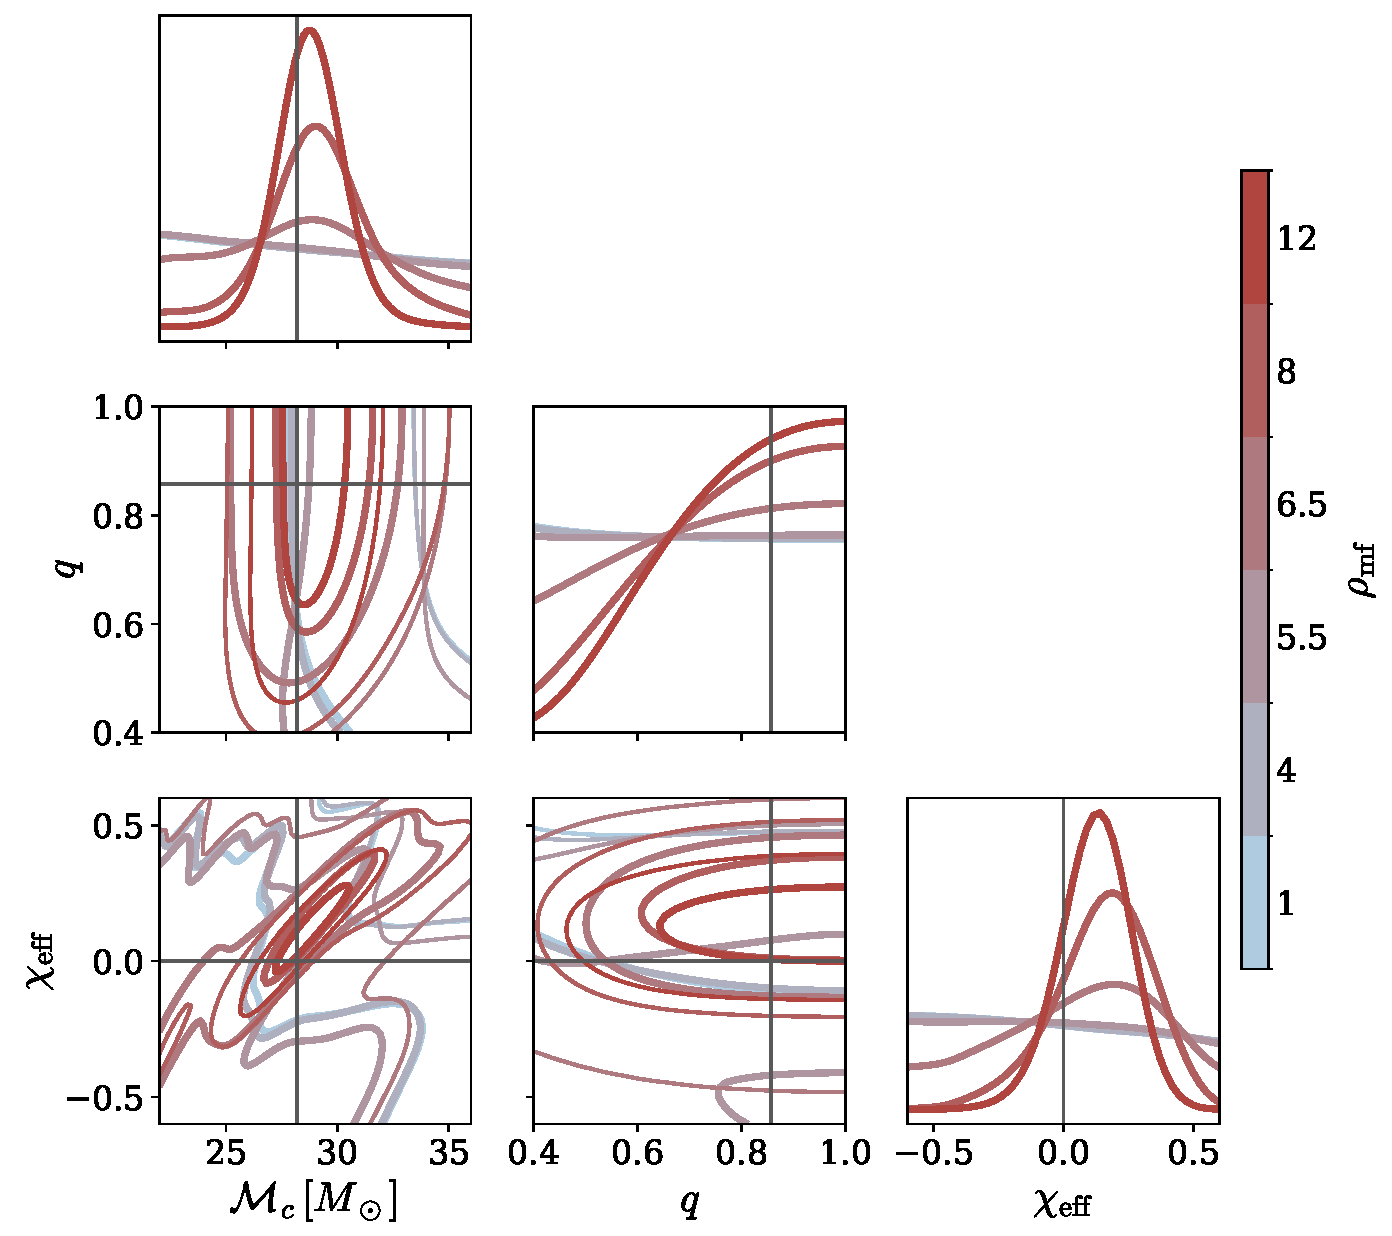
\includegraphics[width=0.46\textwidth]{grid_family.pdf}
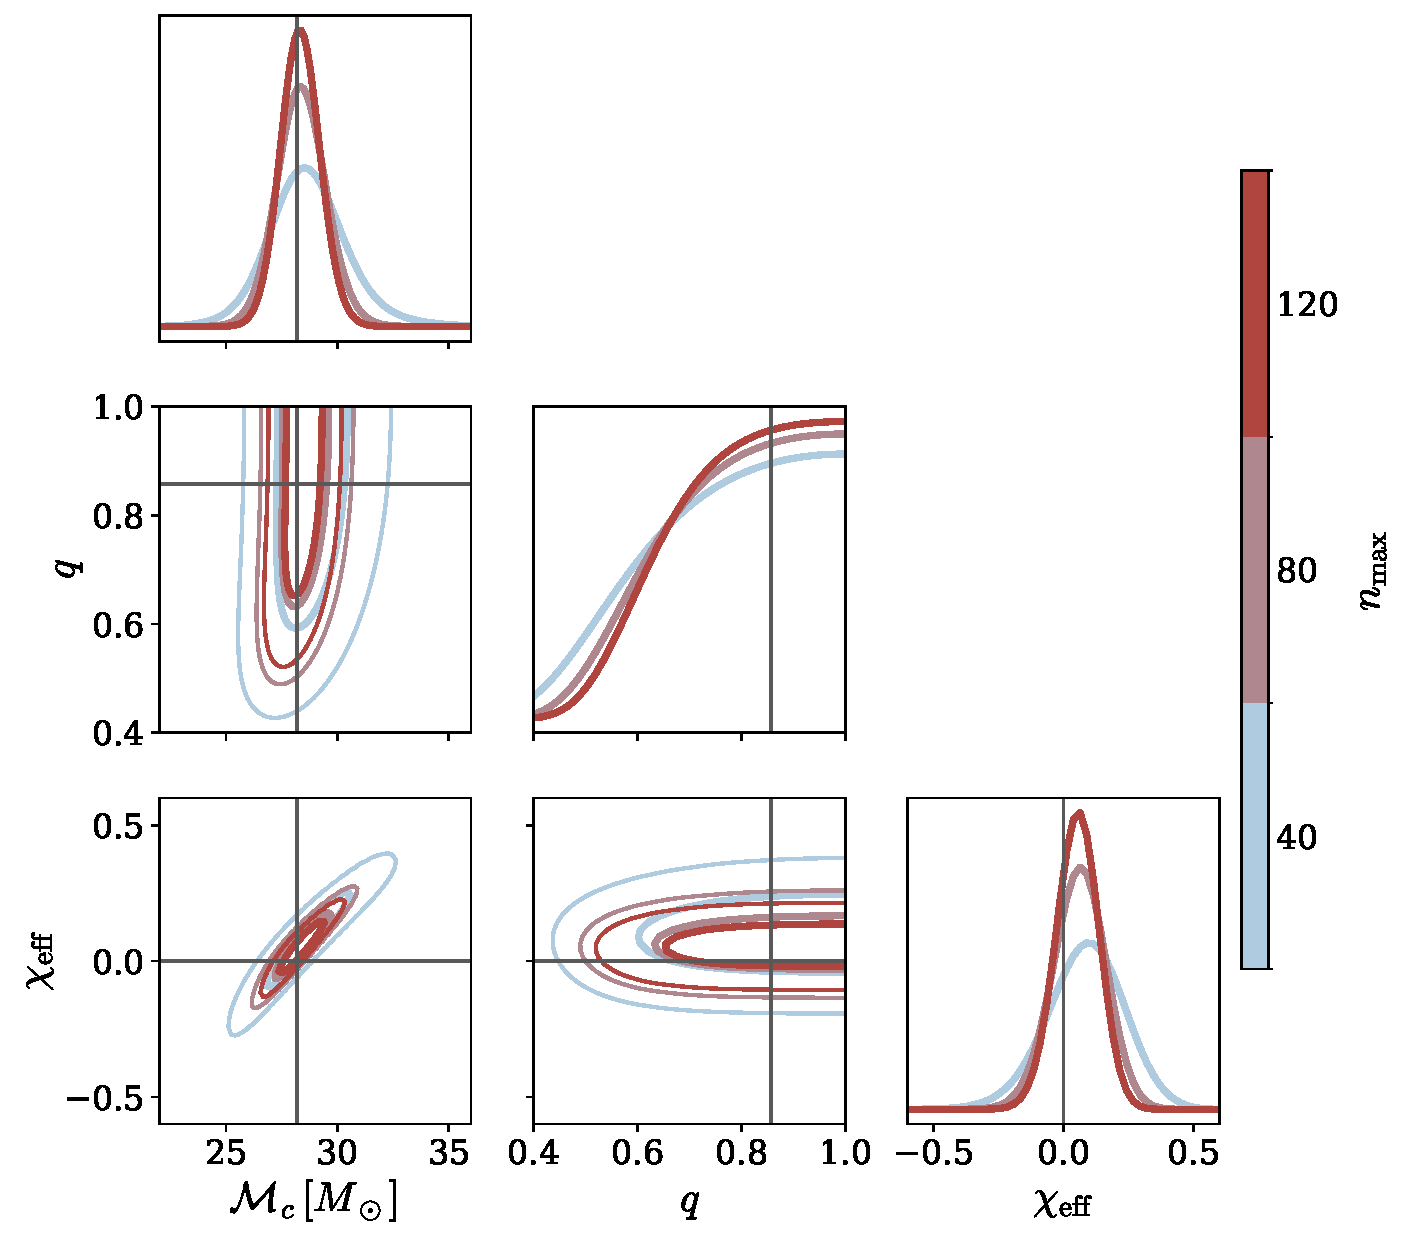
\includegraphics[width=0.46\textwidth]{grid_nmax.pdf}
\caption{Posteriors of one event over its intrinsic parameters. The event is injected at arrival time $t_c = 2.4$ s, sky angles $(\theta, \phi) = (2.27, 4.02)$, polarization $\psi = 1.47$ and inclination $\cos\iota = -0.26$, over which the analysis marginalizes. Left, the SNR varied at fixed $n_{\max} = 40$, from low SNR in light to high SNR in dark. Right, the truncation order $n_{\max}$ varied over 3 values at a fixed matched filter SNR of 25. Contours are the 50 and 90 percent credible regions, and red lines mark the injected values.}
\label{fig:corner}
\end{figure*}

Possible discretization errors of the stored implementation, from the $(|z_1|, |z_2|, \Delta\varphi)$ lattice, the template power grid, and the arrival time sample grid, are investigated in Appendix~\ref{app:construction} and are negligible.

We also check possible biases of the recovered posteriors over
multiple events. We draw 592 injections from the analysis priors
restricted to the controlled domain
$\rho_{\rm mf} \lesssim \sqrt{2 n_{\max}}$, analyze each with
independent noise and no detection threshold at $n_{\max} = 120$, and
calculate the credible level of the injected parameters in each
posterior, to plot the probability probability (PP) curves of
Fig.~\ref{fig:pp}. The Kolmogorov Smirnov (KS) $p$ values are 0.47
for the chirp mass, 0.87 for the mass ratio, and 0.28 for the aligned
spin, all consistent with an unbiased recovery.

\begin{figure}[htb]
\centering
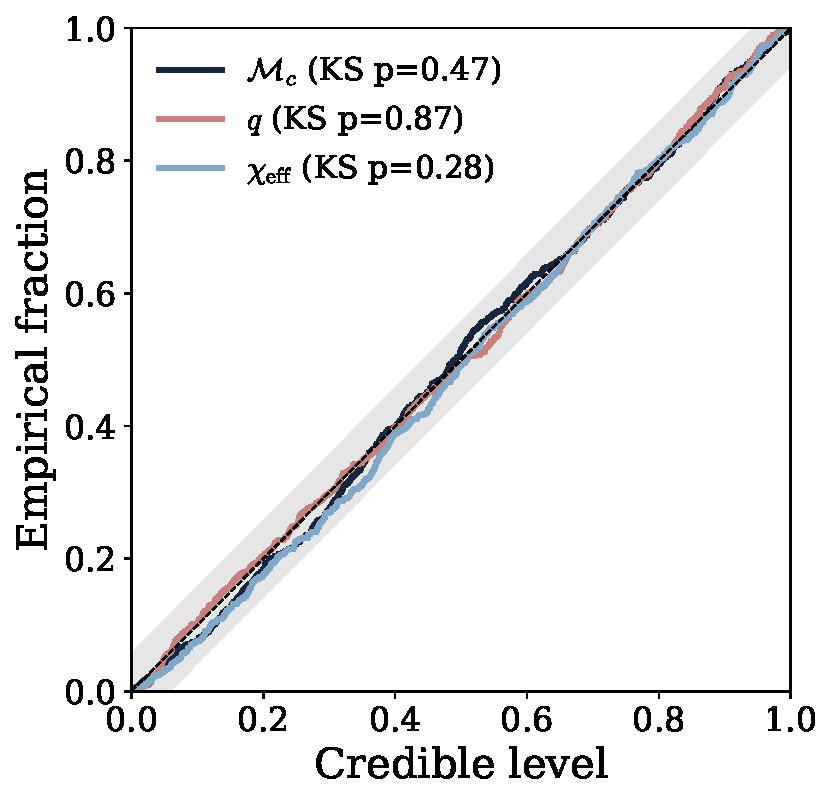
\includegraphics[width=0.42\textwidth]{pp.pdf}
\caption{PP curves over the 592 injections at
$n_{\max} = 120$. The band is the 95 percent KS region.}
\label{fig:pp}
\end{figure}

\section{Background Simulations}
\label{app:simpop}

To demonstrate the search on a realistic intermittent background, we
choose a simple representative population model. BBHs
merge at the rate density $R_0 = 30~{\rm Gpc^{-3}\,yr^{-1}}$, chosen
to be consistent with GWTC-5 \cite{GWTC5}. The detector frame chirp mass follows a power law
plus peak model, the phenomenological form of the LVK population
analyses \cite{GWTC3}, with slope $\alpha = -2.3$, peak fraction
$f_{\rm peak} = 0.1$, peak location $\mu = 30\,M_\odot$, and peak
width $2\,M_\odot$ in the range 10 to 44 $M_\odot$. The mass ratio and
the aligned spin are uniform over their analysis ranges, the angles are
isotropic, and the distance is drawn from the analysis distance prior
itself, in the detector frame, so that the population's distance
distribution matches the prior of the search. The population model
therefore carries 4 free parameters, the rate density $R_0$ and the
mass model $(\alpha, f_{\rm peak}, \mu)$, with the peak width and the
mass ratio and spin distributions held fixed.

We simulate 4 s long data segments in two detectors, LIGO Hanford
and LIGO Livingston, at the A+ design sensitivity
\cite{AplusDesign}. The main set holds $3 \times 10^4$ segments, 33
hours of data, with the event count of every segment drawn from the
Poisson law at the rate $R_0$, together with $3 \times 10^3$ noise
only control segments. A further $1.2 \times 10^5$ segments, 133
hours, hold noise only, and the 20 chunks of the search redraw
the occupancy of this set at the injected rate, replacing every
occupied segment with a draw from the 468 occupied segments of the
main set. Joining the 20 chunks forms the
single observation of 111 days over which
Fig.~\ref{fig:bftime} accumulates the detection statistic. Since the mixture likelihood of
Eq.~\eqref{eq:mixture} is suitable for $\bar N \ll 1$, we also
choose longer segment durations of 8, 32, and 192 s, to deliberately
test the search as overlapping events break this condition. We
simulate the data directly in the frequency domain and inject the
signals with arrival times uniform across the segment.

The intrinsic template grid holds 28 chirp masses, 8 mass ratios,
and 8 aligned spins, 1792 templates in total, evaluated at
$n_{\max} = 120$. The weights of Eq.~\eqref{eq:lbar} are
\begin{equation}
w_k \propto \Big[ (1 - f_{\rm peak})\,
\frac{{\Mc}_k^{\,\alpha}}{N_\alpha}
+ f_{\rm peak}\,
\frac{e^{-({\Mc}_k - \mu)^2 / 2 \sigma_\mu^2}}
{\sqrt{2 \pi}\, \sigma_\mu} \Big]\, \Delta{\Mc}_k,
\label{eq:massmodel}
\end{equation}
with $\sigma_\mu = 2\,M_\odot$,
$N_\alpha = (44^{\alpha+1} - 10^{\alpha+1}) / (\alpha + 1)$ the
power law normalization over the chirp mass range, $\Delta{\Mc}_k$ the
grid measure, the weights normalized to $\sum_k w_k = 1$ and uniform
over the mass ratio and spin axes.

\section{Segment Duration}
\label{app:tseg}

Figure~\ref{fig:tseg} repeats the population fit at segment
durations of 4, 8, 32, and 192 s, with the whole segment searched, so
that both the arrival window and $\bar N$ grow with the duration and
the generation and the fit use the same exposure.

\begin{figure*}[htb]
\centering
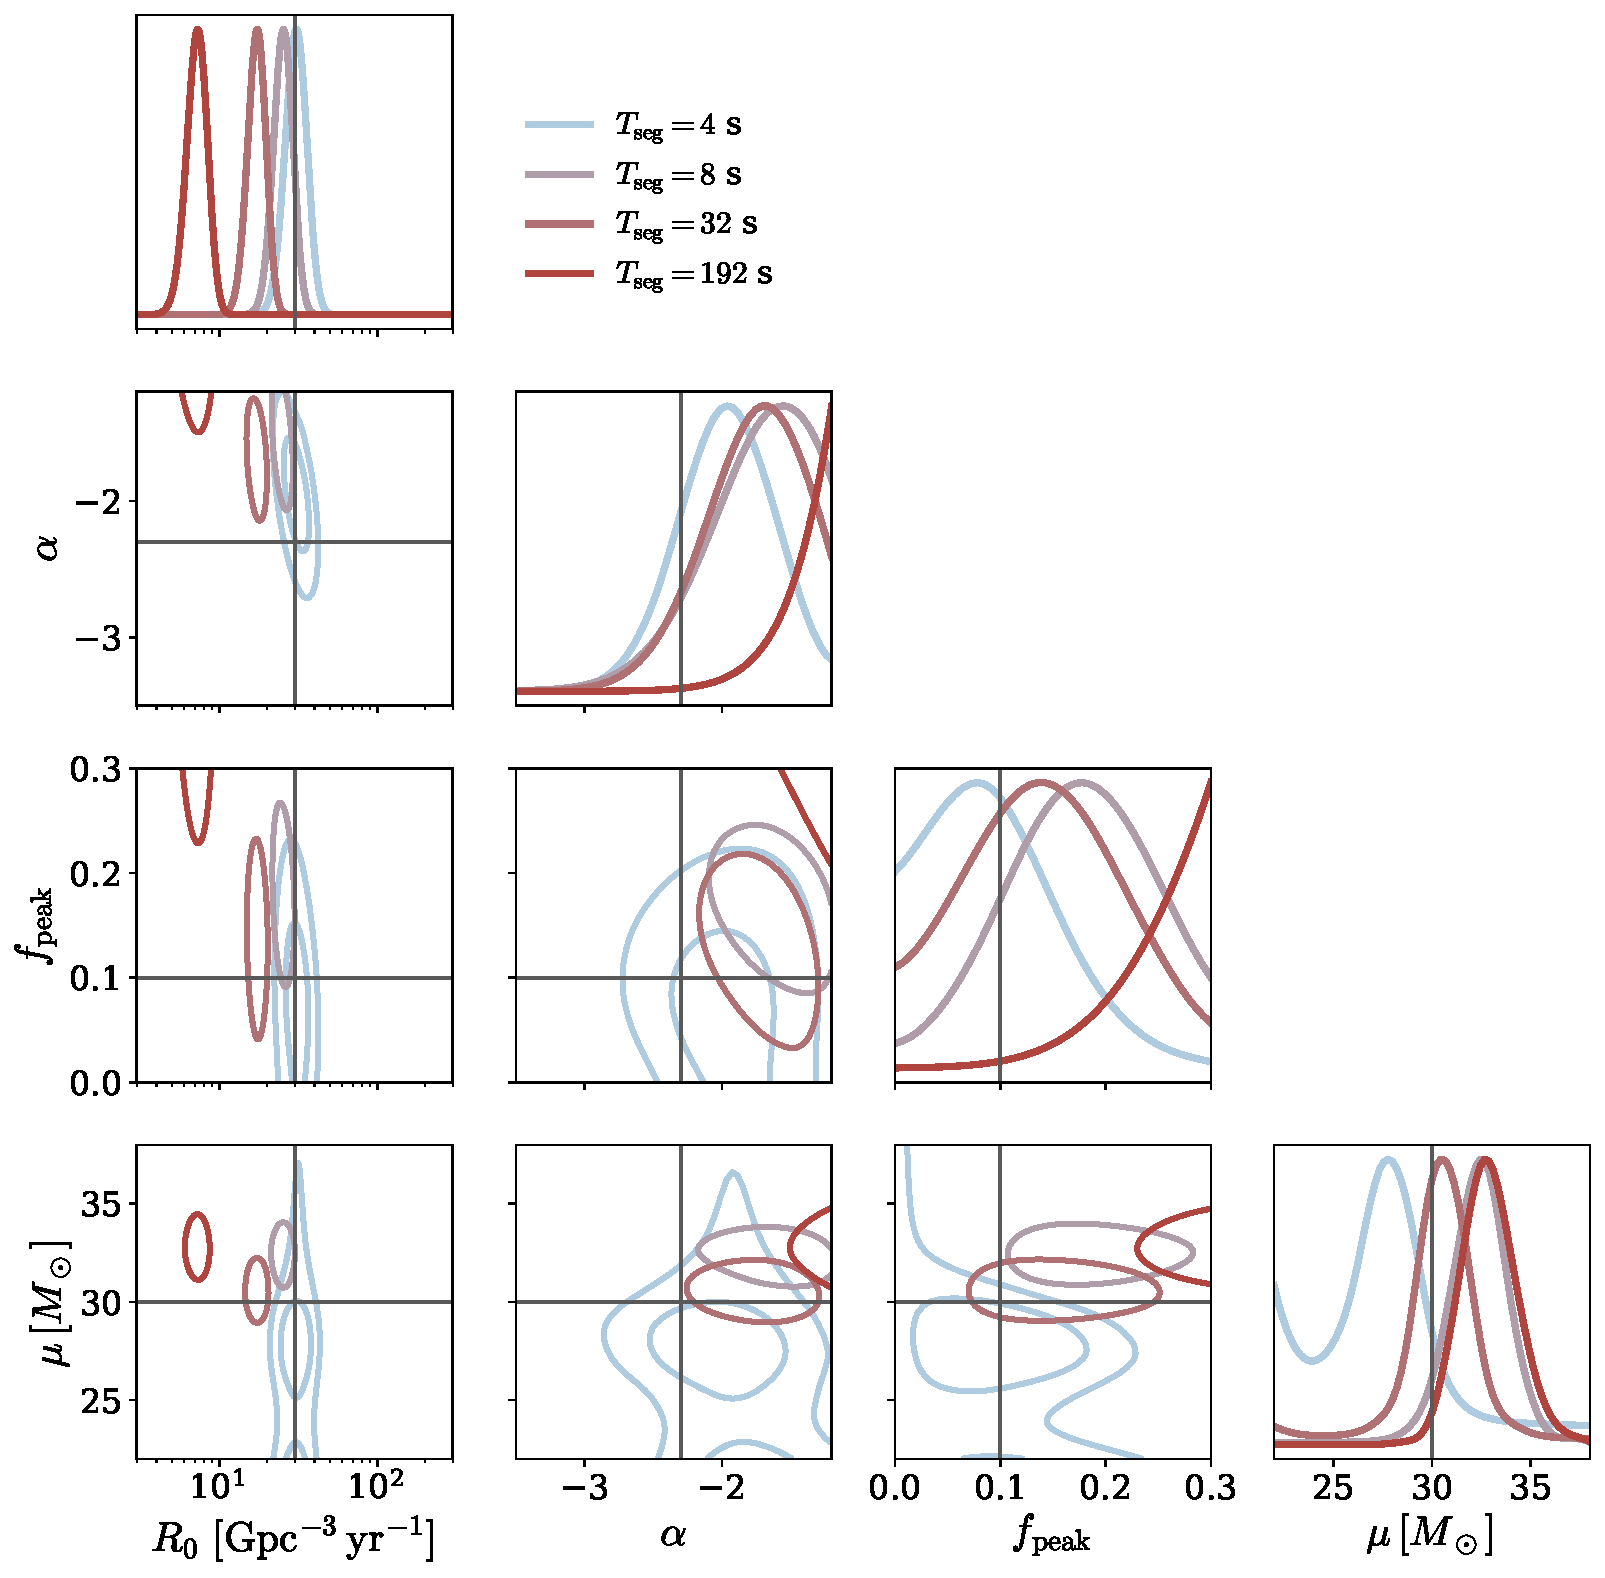
\includegraphics[width=0.62\textwidth]{sgwb_tseg.pdf}
\caption{Population posteriors at segment durations of 4, 8, 32, and
192 s. Longer segments raise the event count per segment and hold
overlapping events that the single event mixture does not model, so
the rate is biased low while the mass peak stays at the injection.
Grey lines mark the injected values.}
\label{fig:tseg}
\end{figure*}


\end{document}
